%  We first introduce the concept of pushout from category theory in \hyperref[preliminaries:pushout]{Section~\ref*{preliminaries:pushout}}. 
%   Next, we discuss the double-pushout (DPO) rewriting in \hyperref[preliminaries:grs]{Section~\ref*{preliminaries:grs}}. 
%   Finally, we explore the concept of relative termination in \hyperref[preliminaries:relative_termination]{Section~\ref*{preliminaries:relative_termination}}. 
%   Additionally, we introduce the notion of a strongly monotonic measurable semiring in \hyperref[sec:strongly_monotonic_measurable_semiring]{Section~\ref*{sec:strongly_monotonic_measurable_semiring}}. 
%   The type graph, which is presented in \hyperref[sec:weighted_type_graph]{Section~\ref*{sec:weighted_type_graph}}, is weighted over this semiring.
  
In this section, we recall definitions related to the double-pushout approach to graph rewriting and relative termination, and we introduce strongly monotonic measurable semirings. For further details, we refer the reader to~\cite{konig2018tutorial,ehrig1997algebraic,habel2001double} for the DPO graph rewriting,~\cite{pierce1991basic, barr1990category} for category theory concepts, and~\cite{geser1990relative} for relative termination.
 
\subsection{Pushout}
\label{preliminaries:pushout}
\todo{Over-formalisation}
% \begin{definition}
%     \label{def:graph:unlabeled}
%     An \textbf{directed unlabeled multigraph} \( G \) consists of 
%     \begin{itemize}
%         \item a collection $V(G)$ of elements, which are called \textbf{nodes} (or \textbf{objects}),
%         \item a collection $E(G)$ of elements different from nodes, which are called \textbf{edges} (or \textbf{arrows}),
%         \item a function $\opn{dom}: E \to V$ assigning to each edge its \textbf{source} (or \textbf{domain}) node,
%         \item a function $\opn{cod}: E \to V$ assigning to each edge its \textbf{target} (or \textbf{codomain}) node.
%     \end{itemize} 
%     An directed unlabeled multigraph $G$ is \textbf{finite} if $V(G)$ and $E(G)$ have both finite elements.
%     Throughout, the term \enquote{unlabeled graph} denotes a directed unlabeled multigraph.
%     We write \( a: s \to t \) to indicate that \( a \) is an edge from \( s \) to \( t \).
% \end{definition}   

% Note that an unlabeled graph can have multiple edges from one node to another, as well as loops (edges from a node to itself), because different edges $u,v$ of the unlabeled graph can have the same source and target nodes, i.e. $\opn{dom}(u) = \opn{dom}(v)$ and $\opn{cod}(u) = \opn{cod}(v)$.


% \begin{example}
%     An unlabeled graph is shown in Figure~\ref{fig:preliminaries:unlabeled_graph}.

%     In an unlabeled graph, edges are directed and will be visualized as arrows; between any two nodes, there can be multiple edges, and loops are allowed. An unlabeled graph is depicted in Figure~\ref{fig:preliminaries:unlabeled_graph} where nodes are marked with numbers to facilitate discussion, but in general, nodes are not labeled.
%     \begin{figure}[H]
%         \centering
%         \begin{tikzpicture}
%             \graphbox{}{0mm}{0mm}{32mm}{28mm}{-10mm}{-14mm}{
%                 \node[draw,circle] (1) at (0,0) {1};
%                 \node[draw,circle] (2) at (2,0) {2};
%                 \draw[->] (1) edge[loop above] (1) ;
%                 \draw[->] (1) edge[loop below] (1) ;
%                 \draw[->] (1) edge[bend left] (2)  ;
%                 \draw[->] (2) edge[bend left] (1)   ;
%             }
%         \end{tikzpicture}
%     \caption{Unlabeled graph}
%     \label{fig:preliminaries:unlabeled_graph}
%     \end{figure}
% \end{example}

% \begin{example}
%     In an unlabeled graph, edges are directed and will be visualized as arrows; between any two nodes, there can be multiple edges, and loops are allowed. An unlabeled graph is depicted in Figure~\ref{fig:preliminaries:unlabeled_graph} where nodes are marked with numbers to facilitate discussion, but in general, nodes are not labeled.
%     \begin{figure}[H]
%         \centering
%         \begin{tikzpicture}
%             \graphbox{}{0mm}{0mm}{32mm}{28mm}{-10mm}{-14mm}{
%                 \node[draw,circle] (1) at (0,0) {1};
%                 \node[draw,circle] (2) at (2,0) {2};
%                 \draw[->] (1) edge[loop above] (1) ;
%                 \draw[->] (1) edge[loop below] (1) ;
%                 \draw[->] (1) edge[bend left] (2)  ;
%                 \draw[->] (2) edge[bend left] (1)   ;
%             }
%         \end{tikzpicture}
%     \caption{Unlabeled graph}
%     \label{fig:preliminaries:unlabeled_graph}
%     \end{figure}
% \end{example}
\begin{definition}[Category \cite{pierce1991basic, barr1990category}]
    \label{def:cat}
    A \textbf{category} is an unlabeled graph \( C \) together with a total function \( u : C_0 \to C_1 \) and a partial function \( \star: C_1 \times C_1 \to C_1 \) such that 
        (i) for all edges \( f:X \to Y \) and \( g:Y \to Z \), the edge \( f \star g :X \to Z \) is defined; 
        (ii) for every node \( X \), \( u(X) \) is an edge from \( X \) to \( X \);
        (iii) for every \( f:X \to Y \), we have \(u(X) \star f = f = f \star u(Y)\);
        (iv) for all edges \( f \), \( g \) and \(h\), we have \( (f \star g) \star h = f \star (g \star h) \) whenever either side is defined.
    Edges are called \textbf{morphisms}. The function $\star$ is called \textbf{composition}. For all \( X \in C_0 \), the edge \( u(X) \) is denoted \( \operatorname{id}_X \) and is called the \textbf{identity} of the object \( X \).
    % \( C \) is called the \textbf{underlying graph} of the category \( \mathcal{C} \).
\end{definition} 
\begin{notation}
    The composition of morphisms \( f : X \mathop{\to} Y \) and \( g : Y \mathop{\to} Z \) is written in diagrammatic order as \( f \mathop{\star} g \), rather than in functional order \( g \circ f \). 
    % The advantage is that, when reading from left to right, the morphisms appear in the same order as in the corresponding diagram, making the notation more intuitive for visual reasoning.
\end{notation}  
\begin{definition}[Monomorphism~\cite{pierce1991basic,barr1990category}]
    \label{def:cat:homo}
    A morphism \( f : X \to Y \) is \textbf{monic} (or a \textbf{monomorphism}) if for all morphisms \( g \) and \( h \), if \( g \star f = h \star f \), then \( g = h \). A monomorphism is denoted by \( f : X \rightarrowtail Y \).
\end{definition} 

\begin{definition}[Span~\cite{lowe2010graph}]
    An ordered pair \( (\alpha : A \mathop{\to} B,~\beta : A \mathop{\to} C) \) of morphisms with a common domain is called a \textbf{span}, denoted by \( B \overset{\alpha}{\leftarrow} A \overset{\beta}{\rightarrow} C \).
\end{definition}

\begin{definition}[Cospan]
    An ordered pair \( (\beta' : B \to D,~\alpha' : C \to D) \) of morphisms with a common codomain is called a \textbf{cospan}, denoted by \( B \overset{\beta'}{\rightarrow} D \overset{\alpha'}{\leftarrow} C \). 
\end{definition} 


\begin{definition}[Diagram \cite{barr1990category}]
    \label{def:cat:diagram}
    Let \( G \) be an unlabeled graph. A \textbf{diagram} (in \( \mathcal{C} \) of shape \( G \)) is a homomorphism of unlabeled graphs \( h : G \to C \) where \( C \) is the underlying unlabeled graph of the category \( \mathcal{C} \). A diagram is \textbf{commutative} if, for all nodes \( u \), \( v \), and any two paths from \( u \) to \( v \) in the unlabeled graph \( G \):

    \begin{center}
    \resizebox{12cm}{!}{
        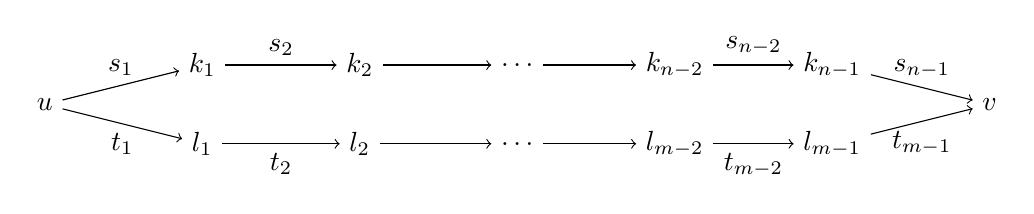
\begin{tikzpicture}
        \node (u) at (0,0) {\( u \)};
        \node (k1) at (2,0.5) {\( k_1 \)};
        \node (k2) at (4,0.5) {\( k_2 \)};
        \node (ketc) at (6,0.5) {\( \dots \)};
        \node (knm2) at (8,0.5) {\( k_{n-2} \)};
        \node (knm1) at (10,0.5) {\( k_{n-1} \)};
        \node (v) at (12,0) {\( v \)};
        \node (l1) at (2,-0.5) {\( l_1 \)};
        \node (l2) at (4,-0.5) {\( l_2 \)};
        \node (letc) at (6,-0.5) {\( \dots \)};
        \node (lnm2) at (8,-0.5) {\( l_{m-2} \)};
        \node (lnm1) at (10,-0.5) {\( l_{m-1} \)};
        \draw[->] (u) -- (k1) node [midway,above] {\( s_1 \)};
        \draw[->] (k1) -- (k2) node [midway,above] {\( s_2 \)};
        \draw[->] (k2) -- (ketc);
        \draw[->] (ketc) -- (knm2); 
        \draw[->] (knm2) -- (knm1) node[midway,above] {\( s_{n-2} \)}; 
        \draw[->] (knm1) -- (v) node[midway,above] {\( s_{n-1} \)}; 
        \draw[->] (u) -- (l1) node[midway,below] {\( t_1 \)};
        \draw[->] (l1) -- (l2) node[midway,below] {\( t_2 \)};
        \draw[->] (l2) -- (letc);
        \draw[->] (letc) -- (lnm2); 
        \draw[->] (lnm2) -- (lnm1) node[midway,below] {\( t_{m-2} \)}; 
        \draw[->] (lnm1) -- (v) node[midway,below] {\( t_{m-1} \)}; 
        \end{tikzpicture}
    }
    \end{center}
    \noindent
    the equality \( h(s_1) \star h(s_2) \star \dots  \star h(s_{n-1}) = h(t_1) \star h(t_2) \star \dots  \star h(t_{m-1}) \) holds.
\end{definition}

Pushouts play a central role in the double-pushout approach to graph rewriting considered in this thesis. The concepts and notation in this section follow the treatments of Pierce~\cite{pierce1991basic} and Barr and Wells~\cite{barr1990category}.
\begin{definition}
    \label{def:cat}
    A \textbf{category}\index{Category} is an unlabeled graph \( C \) together with a total function \( u : V(C)  \mathop{\to} E(C) \) and a partial function \( \star: E(C) \mathop{\times} E(C)  \mathop{\to} E(C) \) such that 
        \begin{itemize}
            \item for all edges \( f:X  \mathop{\to} Y \) and \( g:Y  \mathop{\to} Z \), the edge \( f \mathop{\star} g :X  \mathop{\to} Z \) is defined; 
            \item  for every node \( X \), \( u(X) \) is an edge from \( X \) to \( X \); 
            \item for every \( f:X  \mathop{\to} Y \), we have \(u(X) \mathop{\star} f \mathop{=} f \mathop{=} f \mathop{\star} u(Y)\);
            \item for all edges \( f \), \( g \) and \(h\), we have \( (f \mathop{\star} g) \mathop{\star} h \mathop{=} f \mathop{\star} (g \mathop{\star} h) \) whenever either side is defined.
        \end{itemize}
    Edges are called \textbf{morphisms}\index{Morphism}. The function $\star$ is called \textbf{composition}\index{Composition}. For all \( X \mathop{\in} V(C) \), the edge \( u(X) \) is denoted by \( \operatorname{id}_X \) and is called the \textbf{identity}~\index{Indentity} of the object \( X \).
    % \( C \) is called the \textbf{underlying graph} of the category \( \mathcal{C} \).
\end{definition}    
\begin{definition}
    A category \(\mathcal{C}\) is said to be \textbf{locally small}\index{Category!locally small} if for all objects \(X,Y\) in \(\mathcal{C}\), the collection $\opn{Hom}(X,Y)$\index{hom(@$\opn{Hom}(X,Y)$} of morphisms from \(X\) to \(Y\) is a set (called a \textbf{hom-set})~\index{Hom-set}. For a locally small category, $\opn{Mono}(X,Y)$\index{mono(@$\opn{Mono}(X,Y)$} denotes the set of all monomorphisms from $X$ to $Y$.
\end{definition}
\textbf{Throughout this section, fix a locally small category \( \mathcal{C} \).}
\begin{example}
    Consider the unlabeled graph shown below.
    %  in Figure~\ref{fig:preliminaries:category}. 
     It can be considered as a category where the objects are the nodes and the morphisms are the paths between nodes; composition is path concatenation. The identity of a node is the self-loop of the node. There are at least three morphisms from the left node to itself: the identity morphism (the self-loop), the path that traverses the self-loop twice, and the path that goes to the right node and back. 
        % \begin{figure}[H]
        % \centering
        \begin{center}
            \resizebox{0.4\textwidth}{!}{
        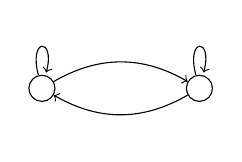
\begin{tikzpicture}
            \graphbox{}{0mm}{0mm}{32mm}{16mm}{-10mm}{-9mm}{
                \node[draw,circle] (1) at (0,0) {};
                \node[draw,circle] (2) at (2,0) {};
                \draw[->] (1) edge[loop above] node[midway, above] { } (1) ;
                \draw[->] (2) edge[loop above] node[midway, above] { } (2) ;
                \draw[->] (1) edge[bend left] node[midway, above] {}  (2)  ;
                \draw[->] (2) edge[bend left] node[midway, below] {} (1)   ;
            }
        \end{tikzpicture}
            }
    %     \caption{}
    %     \label{fig:preliminaries:category}
    % \end{figure}
        \end{center}
\end{example}

% cat notation * 
\begin{notation}
    The composition of morphisms \( f : X  \mathop{\to} Y \) and \( g : Y  \mathop{\to} Z \) is written in diagrammatic order as \( f \mathop{\star} g \), rather than in functional order \( g \circ f \) as is common in litterature. The advantage is that, when reading from left to right, the morphisms appear in the same order as in the corresponding diagram, making the reasoning accompanying diagrams more intuitive. 
\end{notation}  

\begin{definition} 
    \label{def:cat:homo}
    A morphism \( f : X  \mathop{\to} Y \) is said to be a \textbf{monomorphism}\index{Monomorphism} (is \textbf{monic}\index{Monic}) if given any morphisms \( g,h: Z  \mathop{\to} X  \), \( g \mathop{\star} f \mathop{=} h \mathop{\star} f \) implies \( g \mathop{=} h \). 
    In this case, we write $f : X \rightarrowtail Y$\index{a@$\rightarrowtail$} to indicate that $f$ is a monomorphism.
\end{definition} 

When visualizing a monomorphism, we often use $\rightarrowtail$ instead of $\to$ to emphasize that it is monic. For example, a monomorphism of labeled graphs can be represented as follows:
\begin{center}
        \resizebox{0.7\textwidth}{!}{
        \begin{tikzpicture}
            \graphbox{$K$}{40mm}{0mm}{24mm}{15mm}{2mm}{-5mm}{
                \coordinate (o) at (5mm,-3mm); 
                \node[draw,circle] (l1) at ($(o)+(-10mm,0mm)$) {1};
                \node[draw,circle] (l2) at ($(l1)+(1,0)$) {2};
            }    
            \graphbox{$R$}{70mm}{0mm}{45mm}{15mm}{2mm}{-5mm}{
                \coordinate (o) at (-5mm,-3mm); 
                \node[draw,circle] (l1) at ($(o)+(-10mm,0mm)$) {1};
                \node[draw,circle] (l2) at ($(l1)+(3,0)$) {2};
                \node[draw,circle] (l3) at ($(l1)+(1,0)$) {4};
                \node[draw,circle] (l4) at ($(l1)+(2,0)$) {5};
                \draw[->] (l1) -- (l3) node[midway,above] {$a$};
                \draw[->] (l3) -- (l4) node[midway,above] {$b$};
                \draw[->] (l4) -- (l2) node[midway,above] {$a$};
            }    
            \node () at (67mm,-8mm) {$\rightarrowtail$};
        \end{tikzpicture}
        }
    \end{center}

\begin{example}
    \index{set@\(\mathbf{Set}\)}\index{Category!set}
The category \(\mathbf{Set}\) has sets as objects and total functions between them as morphisms. For \(f\mathop{\colon} A \mathop{\to} B\) and \(g\mathop{\colon} B \mathop{\to} C\), composition is given by \(g\circ f\), and the identity morphism on a set \(A\) is the identity function \(\mathrm{id}_A\).
\end{example}

\begin{example} 
    Finite labeled graphs and their homomorphisms form a category, hereafter denoted by \textbf{Graph}\index{graph@\textbf{Graph}}\index{Category!graph}. Its objects are labeled graphs, its morphisms are graph homomorphisms, and the monomorphisms are homomorphisms. 
    $\textbf{Graph}$ is locally small. 
\end{example}

% \begin{definition}[Span \cite{lowe2010graph}]
%     A pair \( (\alpha : A  \mathop{\to} B,~\beta : A  \mathop{\to} C) \) of morphisms with a common domain is called a \textbf{span}, denoted by \( B \overset{\alpha}{\leftarrow} A \overset{\beta}{\rightarrow} C \).
% \end{definition}
 
% \begin{definition}[Cospan]
%     A pair \( (\beta' : B  \mathop{\to} D,~\alpha' : C  \mathop{\to} D) \) of morphisms with a common codomain is called a \textbf{cospan}, denoted by \( B \overset{\beta'}{\rightarrow} D \overset{\alpha'}{\leftarrow} C \). 
% \end{definition} 
A span (resp. cospan) is a couple of morphisms with a common domain (resp. codomain).
\begin{definition}
An ordered pair \((\alpha : A  \mathop{\to} B,\, \beta : A  \mathop{\to} C)\) of morphisms with a common domain is called a \textbf{span}\index{Span} \cite{lowe2010graph}, denoted by
\(
B \overset{\alpha}{\leftarrow} A \overset{\beta}{\rightarrow} C
\). 
% An example of a span $(\alpha, \beta)$ is shown below.
Likewise, an ordered pair \((\beta' : B  \mathop{\to} D,\, \alpha' : C  \mathop{\to} D)\) of morphisms with a common codomain is called a \textbf{cospan}\index{Cospan}, denoted by
\(
B \overset{\beta'}{\rightarrow} D \overset{\alpha'}{\leftarrow} C
\). 
\end{definition}
\begin{example}
Consider the diagram below in the category \textbf{Graph}, where the numbers inside nodes and the subgraphs in different colors illustrate how the morphisms map nodes and edges. $(\alpha, \beta)$ is a span, and $(\beta', \alpha')$ is a cospan.


\begin{center}
        \resizebox{0.8\textwidth}{!}{
        \begin{tikzpicture} 
            \graphbox{\( L \)}{40mm}{20mm}{34mm}{12mm}{2mm}{2mm}{
                \coordinate (o) at (0mm,-8mm); 
                \node[draw,circle] (l1) at ($(o)+(-10mm,0mm)$) {1};
                \node[draw,circle] (l2) at ($(l1)+(2,0)$) {2};
                \node[draw,circle,red] (l3) at ($(l1)+(1,0)$) {3};
                \draw[->,red] (l1) -- (l3) node[midway,above] {$a$};
                \draw[->,red] (l3) -- (l2) node[midway,above] {$a$};
            } 
    
            \graphbox{\( K \)}{0mm}{0mm}{34mm}{12mm}{2mm}{2mm}{
                \coordinate (o) at (0mm,-8mm); 
                \node[draw,circle] (l1) at ($(o)+(-10mm,0mm)$) {1};
                \node[draw,circle] (l2) at ($(l1)+(2,0)$) {2};
            }  
            \graphbox{\(G\)}{90mm}{5mm}{34mm}{24mm}{2mm}{-3mm}{
                \coordinate (o) at (0mm,-5mm); 
                \node[draw,circle] (l1) at ($(o)+(-10mm,0mm)$) {1};
                \node[draw,circle] (l2) at ($(l1)+(2,0)$) {2};
                \node[draw,circle,red] (l3) at ($(l1)+(1,0)$) {3};
                \node[draw,circle,blue] (l4) at ($(l2)+(0,-1)$) {6};
                \draw[->,red] (l1) -- (l3) node[midway,above] {$a$};
                \draw[->,red] (l3) -- (l2) node[midway,above] {$a$};
                \draw[->,blue] (l2) -- (l4) node[midway,right] {$a$};
                \node[draw,circle,blue] (l6) at ($(l1)+(0,-1)$) {7};
                \draw[<-,blue] (l1) -- (l6) node[midway,left] {$a$};
                \draw[->,blue] (l2) edge[out=-135,in=-45]node[midway,below] {$a$} (l1) ;
            }   
     
            \graphbox{\( C \)}{40mm}{-20mm}{34mm}{24mm}{2mm}{-3mm}{
                \coordinate (o) at (0mm,-5mm); 
                \node[draw,circle] (l1) at ($(o)+(-10mm,0mm)$) {1};
                \node[draw,circle] (l2) at ($(l1)+(2,0)$) {2};
                \node[draw,circle,blue] (l4) at ($(l2)+(0,-1)$) {6};
                \draw[->,blue] (l2) -- (l4) node[midway,right] {$a$};
                \draw[->,blue] (l2) edge[out=-135,in=-45]node[midway,below] {$a$} (l1) ;
                \node[ draw,circle,blue] (l6) at ($(l1)+(0,-1)$) {7};
                \draw[<-,blue] (l1) -- (l6) node[midway,left] {$a$};
            }      
            % K to L
            \draw[->] (17mm,5mm) -- node[above] {$\alpha$} (37mm,15mm);
            % C to G
            \draw[->] (76mm,-28mm)-- node[below] {$\alpha'$} (104mm,-21mm) ;
            % K to C
            \draw[->] (17mm,-17mm) -- node[below] {$\beta$} (37mm,-28mm);
            % L to G
            \draw[->] (76mm,16mm) -- node[above] {$\beta'$} (104mm,7mm);
            % \node () at (57mm,-6mm) {$PO$};
        \end{tikzpicture}
        }
    \end{center}
\end{example}

\begin{definition}[\cite{barr1990category}]
    \label{def:cat:diagram}
    Let $\mathcal{C}$ be a category, and \( G \) an unlabeled graph. A \textbf{diagram}\index{Diagram} (of shape \( G \)) is a homomorphism of unlabeled graphs \( h : G  \mathop{\to} \mathcal{C} \) where \( \mathcal{C} \) is considered as an unlabeled graph. A diagram is said to be \textbf{commutative}\index{Diagram!commutative} if, for all nodes \( u \), \( v \), and any two paths from \( u \) to \( v \) in the unlabeled graph \( G \):

    \begin{center}
    \resizebox{12cm}{!}{
        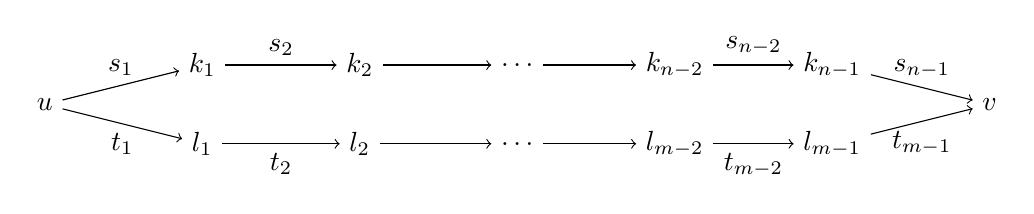
\begin{tikzpicture}
        \node (u) at (0,0) {\( u \)};
        \node (k1) at (2,0.5) {\( k_1 \)};
        \node (k2) at (4,0.5) {\( k_2 \)};
        \node (ketc) at (6,0.5) {\( \dots \)};
        \node (knm2) at (8,0.5) {\( k_{n-2} \)};
        \node (knm1) at (10,0.5) {\( k_{n-1} \)};
        \node (v) at (12,0) {\( v \)};
        \node (l1) at (2,-0.5) {\( l_1 \)};
        \node (l2) at (4,-0.5) {\( l_2 \)};
        \node (letc) at (6,-0.5) {\( \dots \)};
        \node (lnm2) at (8,-0.5) {\( l_{m-2} \)};
        \node (lnm1) at (10,-0.5) {\( l_{m-1} \)};
        \draw[->] (u) -- (k1) node [midway,above] {\( s_1 \)};
        \draw[->] (k1) -- (k2) node [midway,above] {\( s_2 \)};
        \draw[->] (k2) -- (ketc);
        \draw[->] (ketc) -- (knm2); 
        \draw[->] (knm2) -- (knm1) node[midway,above] {\( s_{n-2} \)}; 
        \draw[->] (knm1) -- (v) node[midway,above] {\( s_{n-1} \)}; 
        \draw[->] (u) -- (l1) node[midway,below] {\( t_1 \)};
        \draw[->] (l1) -- (l2) node[midway,below] {\( t_2 \)};
        \draw[->] (l2) -- (letc);
        \draw[->] (letc) -- (lnm2); 
        \draw[->] (lnm2) -- (lnm1) node[midway,below] {\( t_{m-2} \)}; 
        \draw[->] (lnm1) -- (v) node[midway,below] {\( t_{m-1} \)}; 
        \end{tikzpicture}
    }
    \end{center}
    \noindent
    the equality \( h(s_1) \mathop{\star} h(s_2) \mathop{\star} \dots  \mathop{\star} h(s_{n-1}) \mathop{=} h(t_1) \mathop{\star} h(t_2) \mathop{\star} \dots  \mathop{\star} h(t_{m-1}) \) holds.
\end{definition}

\begin{example}
    A commutative diagram in the category \textbf{Graph} of finite, directed, edge-labeled multigraphs is illustrated below. The numbers inside nodes and the subgraphs in different colors illustrate how the morphisms map nodes and edges. 
     The symbol $\mathop{=}$ in the center of the diagram
    is used to indicate that the diagram is commutative,
    i.e. the composition of morphisms along every path from node 1 to node 2 is the same.
    \begin{center}
        \resizebox{0.8\textwidth}{!}{
        \begin{tikzpicture} 
            \graphbox{\( L \)}{40mm}{20mm}{34mm}{12mm}{2mm}{2mm}{
                \coordinate (o) at (0mm,-8mm); 
                \node[draw,circle] (l1) at ($(o)+(-10mm,0mm)$) {1};
                \node[draw,circle] (l2) at ($(l1)+(2,0)$) {2};
                \node[draw,circle,red] (l3) at ($(l1)+(1,0)$) {3};
                \draw[->,red] (l1) -- (l3) node[midway,above] {$a$};
                \draw[->,red] (l3) -- (l2) node[midway,above] {$a$};
            } 
    
            \graphbox{\( K \)}{0mm}{0mm}{34mm}{12mm}{2mm}{2mm}{
                \coordinate (o) at (0mm,-8mm); 
                \node[draw,circle] (l1) at ($(o)+(-10mm,0mm)$) {1};
                \node[draw,circle] (l2) at ($(l1)+(2,0)$) {2};
            }  
            \graphbox{\(G\)}{90mm}{5mm}{34mm}{24mm}{2mm}{-3mm}{
                \coordinate (o) at (0mm,-5mm); 
                \node[draw,circle] (l1) at ($(o)+(-10mm,0mm)$) {1};
                \node[draw,circle] (l2) at ($(l1)+(2,0)$) {2};
                \node[draw,circle,red] (l3) at ($(l1)+(1,0)$) {3};
                \node[draw,circle,blue] (l4) at ($(l2)+(0,-1)$) {6};
                \draw[->,red] (l1) -- (l3) node[midway,above] {$a$};
                \draw[->,red] (l3) -- (l2) node[midway,above] {$a$};
                \draw[->,blue] (l2) -- (l4) node[midway,right] {$a$};
                \node[draw,circle,blue] (l6) at ($(l1)+(0,-1)$) {7};
                \draw[<-,blue] (l1) -- (l6) node[midway,left] {$a$};
                \draw[->,blue] (l2) edge[out=-135,in=-45]node[midway,below] {$a$} (l1) ;
            }   
     
            \graphbox{\( C \)}{40mm}{-20mm}{34mm}{24mm}{2mm}{-3mm}{
                \coordinate (o) at (0mm,-5mm); 
                \node[draw,circle] (l1) at ($(o)+(-10mm,0mm)$) {1};
                \node[draw,circle] (l2) at ($(l1)+(2,0)$) {2};
                \node[draw,circle,blue] (l4) at ($(l2)+(0,-1)$) {6};
                \draw[->,blue] (l2) -- (l4) node[midway,right] {$a$};
                \draw[->,blue] (l2) edge[out=-135,in=-45]node[midway,below] {$a$} (l1) ;
                \node[ draw,circle,blue] (l6) at ($(l1)+(0,-1)$) {7};
                \draw[<-,blue] (l1) -- (l6) node[midway,left] {$a$};
            }      
            % K to L
            \draw[->] (17mm,5mm) -- node[above] {$\alpha$} (37mm,15mm);
            % C to G
            \draw[->] (76mm,-28mm)-- node[below] {$\alpha'$} (104mm,-21mm) ;
            % K to C
            \draw[->] (17mm,-17mm) -- node[below] {$\beta$} (37mm,-28mm);
            % L to G
            \draw[->] (76mm,16mm) -- node[above] {$\beta'$} (104mm,7mm);
            \node () at (57mm,-6mm) {$\mathop{=}$};
        \end{tikzpicture}
        }
    \end{center}
\end{example}

\begin{notation}   
    When the context makes it clear, \( h_{AB} \) denotes a morphism \( h : A  \mathop{\to} B \), and we refer to diagrams by listing their nodes, as is standard in geometry. 
    % For example, the diagram shown in Definition~\ref{def:cat:po} is denoted by \( ACDB \) or \( ABDC \).
\end{notation}   

The pushout is a construction in category theory that can often be thought of as the construction of a new structure from two given structures by gluing them along a common interface structure.
\begin{definition}
    \label{def:cat:po} 
    A \textbf{pushout}\index{Pushout} of a span \( B \overset{\alpha}{\leftarrow} A \overset{\beta}{\rightarrow} C \), shown in the following diagram,
    %  in Figure~\ref{fig:preliminaries:pushout_sdfkjasdlgjfl}
    is defined as a cospan \( B \overset{\beta'}{\rightarrow} D \overset{\alpha'}{\leftarrow} C \) such that the following conditions hold:
    \begin{itemize}
        \item \( \alpha \mathop{\star} \beta' \mathop{=} \beta \mathop{\star} \alpha' \),
        \item for every cospan \( B \overset{\gamma'}{\rightarrow} E \overset{\gamma}{\leftarrow} C \), if \( \alpha \mathop{\star} \gamma' \mathop{=} \beta \mathop{\star} \gamma \) holds, then there is a unique morphism \(\delta : D  \mathop{\to} E\) such that \( \gamma' \mathop{=} \beta' \mathop{\star} \delta \) and \( \gamma \mathop{=} \alpha' \mathop{\star} \delta \).
    \end{itemize} 
    \begin{center}
        \resizebox{0.45\textwidth}{!}{
            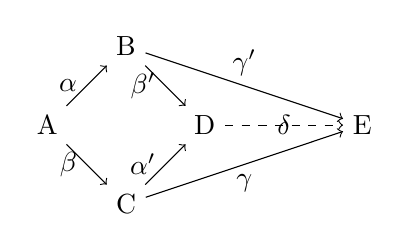
\begin{tikzpicture}
                    \node (i) at (0,0) {A};
                    \node (r) at (1,1) {B};
                    \node (c) at (1,-1) {C};
                    \node (h) at (2,0) {D};
                    % \node () at (1,-1) {\( \Delta \)};
                    \draw[->]  (i) -- (r) node [midway,left] {$ \alpha $};
                    \draw[->] (c) -- (h) node [midway,left] {$ \alpha' $};
                    \draw[->] (r) -- (h) node[midway, left] {$ \beta' $};
                    \draw[->] (i) -- (c) node[midway, left] {$ \beta $};
                    \node (d') at (4,0) {E};
                    \draw[->] (c) -- (d') node [midway,below]{$ \gamma $};
                    \draw[->] (r) -- (d') node [midway,above]{$ \gamma' $};
                    \draw[->,dashed] (h) -- (d') node [midway]{$ \delta $};
                \end{tikzpicture}
        }
            \end{center}
The diagram involving \( (\alpha, \beta, \alpha', \beta') \) is called a \textbf{pushout square}\index{Pushout!square}, or simply a \textbf{pushout}, with \(D\) as the \textbf{pushout object}\index{Pushout!object}. The existence of a unique morphism is known as the \textbf{universal mapping property of the pushout}\index{Pushout!universal mapping property}.
\end{definition} 

\begin{example}
    \label{ex:cat:posfjsdlkgja}
     Pushouts of a span always exist in \(\mathbf{Set}\), and (up to isomorphism) can be described as follows. Let
    \( B \overset{\alpha}{\leftarrow} A \overset{\beta}{\rightarrow} C \) be a span. Its pushout is the cospan \( B \overset{\beta'}{\rightarrow} D \overset{\alpha'}{\leftarrow} C \) where the pushout object of \((\alpha,\beta)\) is the quotient set
    \[
    D \;=\; (B\mathop{+}C)/{\sim}
    \]
    where \(B\mathop{+}C\) denotes the disjoint union of $B$ and $C$ and \(\sim\) is the smallest equivalence relation that includes \(\set{(\alpha(a),\beta(b))\mid a \mathop{\in} A }\). The maps
    \(\beta' \mathop{\colon} B \mathop{\to} D\) and \(\alpha' \mathop{\colon} C \mathop{\to} D\) send each element to its equivalence class.

    For example, consider the functions \(\alpha\) and \(\beta\) in the category \(\mathbf{Set}\) in the diagram, illustrated in Figure~\ref{fig:preliminaries:a_rewriting_step_dfjalsdkjflg}.
    In this diagram, each set is drawn as a box and its elements are represented by circles. The numbers inside circles indicate how the functions map those elements.
    \begin{figure}[H]
      \centering 
      \resizebox{0.6\textwidth}{!}{
      \begin{tikzpicture}
          \graphbox{\( A\)}{40mm}{-3mm}{34mm}{12mm}{2mm}{2mm}{
              \coordinate (o) at (0mm,-8mm); 
              \node[draw,circle] (l1) at ($(o)+(-10mm,0mm)$) {1};
              \node[draw,circle] (l2) at ($(l1)+(2,0)$) {2};
          }  
          \graphbox{\( B \)}{80mm}{-3mm}{45mm}{12mm}{2mm}{2mm}{
              \coordinate (o) at (-5mm,-8mm); 
              \node[draw,circle] (l1) at ($(o)+(-10mm,0mm)$) {1};
              \node[draw,circle] (l2) at ($(l1)+(3,0)$) {2};
              \node[draw,circle] (l3) at ($(l1)+(1,0)$) {4};
          }     
          \graphbox{\( C  \)}{40mm}{-22mm}{34mm}{22mm}{2mm}{-3mm}{
              \coordinate (o) at (0mm,-3mm); 
              \node[draw,circle] (l1) at ($(o)+(-10mm,0mm)$) {1};
              \node[draw,circle] (l2) at ($(l1)+(2,0)$) {2};
              \node[ draw,circle] (l6) at ($(l1)+(0,-1)$) {3};
          }    
          \graphbox{\( D \)}{80mm}{-22mm}{45mm}{22mm}{2mm}{-3mm}{
              \coordinate (o) at (-5mm,-3mm); 
              \node[draw,circle] (l1) at ($(o)+(-10mm,0mm)$) {1};
              \node[draw,circle] (l2) at ($(l1)+(3,0)$) {2};
              \node[draw,circle] (l3) at ($(l1)+(1,0)$) {4};
              \node[ draw,circle] (l6) at ($(l1)+(0,-1)$) {3};
          }    
          \node () at (77mm,-8mm) {\( \overset{\alpha}{\rightarrow} \)}; % K -> R
          \node () at (58mm,-18mm) {\( \beta\downarrow \)};
          \node () at (102mm,-18mm) {\( \beta'\downarrow \)};
          \node () at (77mm,-33mm) {\( \overset{\alpha'}{\rightarrow} \)}; % C -> H
      \end{tikzpicture}
      }
      \caption{}
      \label{fig:preliminaries:a_rewriting_step_dfjalsdkjflg}
  \end{figure}
    Throughout this example, an element labeled \(n\) in a set \(X\) is denoted by \(n_X\) to avoid ambiguity.        
    The binary relation \(\sim\) is the reflexive, symmetric and transitive closure of the binary relation $\{(1_B,1_C),(2_B,2_C)\}$.
 
    The disjoint union of \(B\) and \(C\) is
    \[ 
    D' \mathop{=} \{1_B,2_B,4_B,1_C,2_C,3_C\},
    \]
    and the quotient set is
    \[
    D'/\sim \mathop{=} \{[1_B],[2_B],[3_C],[4_B]\},
    \]
    where $[x]$ denotes the equivalence class of the element \(x\).
    We have \([1_C]=[1_B]\) and \([2_C]=[2_B]\), and the maps
    \(\beta'' \mathop{\colon} B \mathop{\to} D'\) and \(\alpha'' \mathop{\colon} C \mathop{\to} D'\) send each element to its equivalence class. Note that \(\{[1_B],[2_B],[3_C],[4_B]\}\) is isomorphic to \(D\), shown in Figure~\ref{fig:preliminaries:a_rewriting_step_dfjalsdkjflg}, which is expected because the pushout of a span is unique up to isomorphism.
\end{example}

\begin{proposition}{\cite[p.188]{corradini1997algebraic}}
    \label{prop:pushout_graph_always_exists}
    In category \textbf{Graph}, the pushout of two arrows always exists: It can be computed componentwise (as a pushout in \textbf{Set}) for the nodes and for the edges, and the source, target, and labeling mappings are uniquely determined.
\end{proposition}

\begin{example}
    The diagram in the category \textbf{Graph} shown below
    %  in Figure~\ref{fig:preliminaries:pushout_injective} 
     is a pushout square. The numbers inside nodes and the subgraphs in different colors illustrate how the morphisms map nodes and edges. In this example, both $\alpha$ and $\beta$ are injective morphisms. Therefore, the pushout object $G$ can be constructed easily by taking the interface graph $K$ and adding elements from $L$ and $C$ which are not present in $K$.
    % \begin{figure}[H]
    %     \centering
    \begin{center}
        \resizebox{0.8\textwidth}{!}{
        \begin{tikzpicture} 
            \graphbox{\( L \)}{40mm}{15mm}{34mm}{12mm}{2mm}{2mm}{
                \coordinate (o) at (0mm,-8mm); 
                \node[draw,circle] (l1) at ($(o)+(-10mm,0mm)$) {1};
                \node[draw,circle] (l2) at ($(l1)+(2,0)$) {2};
                \node[draw,circle,red] (l3) at ($(l1)+(1,0)$) {3};
                \draw[->,red] (l1) -- (l3) node[midway,above] {$a$};
                \draw[->,red] (l3) -- (l2) node[midway,above] {$a$};
            } 
    
            \graphbox{\( K \)}{0mm}{0mm}{34mm}{12mm}{2mm}{2mm}{
                \coordinate (o) at (0mm,-8mm); 
                \node[draw,circle] (l1) at ($(o)+(-10mm,0mm)$) {1};
                \node[draw,circle] (l2) at ($(l1)+(2,0)$) {2};
            }  
            \graphbox{\(G  \)}{90mm}{5mm}{34mm}{24mm}{2mm}{-3mm}{
                \coordinate (o) at (0mm,-5mm); 
                \node[draw,circle] (l1) at ($(o)+(-10mm,0mm)$) {1};
                \node[draw,circle] (l2) at ($(l1)+(2,0)$) {2};
                \node[draw,circle,red] (l3) at ($(l1)+(1,0)$) {3};
                \node[draw,circle,blue] (l4) at ($(l2)+(0,-1)$) {6};
                \draw[->,red] (l1) -- (l3) node[midway,above] {$a$};
                \draw[->,red] (l3) -- (l2) node[midway,above] {$a$};
                \draw[->,blue] (l2) -- (l4) node[midway,right] {$a$};
                \node[draw,circle,blue] (l6) at ($(l1)+(0,-1)$) {7};
                \draw[<-,blue] (l1) -- (l6) node[midway,left] {$a$};
                \draw[->,blue] (l2) edge[out=-135,in=-45]node[midway,below] {$a$} (l1) ;
            }   
     
            \graphbox{\( C \)}{40mm}{-15mm}{34mm}{24mm}{2mm}{-3mm}{
                \coordinate (o) at (0mm,-5mm); 
                \node[draw,circle] (l1) at ($(o)+(-10mm,0mm)$) {1};
                \node[draw,circle] (l2) at ($(l1)+(2,0)$) {2};
                \node[draw,circle,blue] (l4) at ($(l2)+(0,-1)$) {6};
                \draw[->,blue] (l2) -- (l4) node[midway,right] {$a$};
                \draw[->,blue] (l2) edge[out=-135,in=-45]node[midway,below] {$a$} (l1) ;
                \node[ draw,circle,blue] (l6) at ($(l1)+(0,-1)$) {7};
                \draw[<-,blue] (l1) -- (l6) node[midway,left] {$a$};
            }      
            % K to L
            \draw[>->] (17mm,5mm) -- node[above] {$\alpha$} (37mm,10mm);
            % C to G
            \draw[>->] (76mm,-28mm)-- node[below] {$\alpha'$} (104mm,-21mm) ;
            % K to C
            \draw[>->] (17mm,-17mm) -- node[below] {$\beta$} (37mm,-28mm);
            % L to G
            \draw[>->] (76mm,10mm) -- node[above] {$\beta'$} (104mm,7mm);
            \node () at (57mm,-6mm) {$PO$};
        \end{tikzpicture}
        }
    \end{center}
    %     \caption{Pushout square with injective morphisms.}
    %     \label{fig:preliminaries:pushout_injective}
    % \end{figure}
\end{example}

\begin{example}
    \label{ex:cat:pushout_non_injective_ssss}
    Consider the diagram in the category \textbf{Graph} shown below, where the numbers inside nodes and the subgraphs in different colors illustrate how the morphisms map nodes and edges. 
    % The diagram 
    % in Figure~\ref{fig:preliminaries:pushout_non_injective} is a pushout square in the category \textbf{Graph}. 
    In this example, $\beta$ is not injective. Therefore, some elements are merged in the pushout object $G$.

    % \begin{figure}[H]
    %     \centering 
    \begin{center}
        \resizebox{0.8\textwidth}{!}{
        \begin{tikzpicture} 
            \graphbox{\( L \)}{40mm}{20mm}{34mm}{20mm}{2mm}{2mm}{
                \coordinate (o) at (0mm,-11mm); 
                \node[draw,circle] (l1) at ($(o)+(-10mm,0mm)$) {1};
                \node[draw,circle] (l2) at ($(l1)+(2,0)$) {2};
                \draw[->,red] (l2) edge[out=-135,in=-45]node[midway,below] {$a$} (l1) ;
                \node[draw,circle,red] (l3) at ($(l1)+(1,0)$) {3};
                \draw[->,red] (l1) -- (l3) node[midway,above] {$a$};
                \draw[->,red] (l3) -- (l2) node[midway,above] {$a$};
            } 
    
            \graphbox{\( K \)}{0mm}{0mm}{34mm}{12mm}{2mm}{2mm}{
                \coordinate (o) at (0mm,-8mm); 
                \node[draw,circle] (l1) at ($(o)+(-10mm,0mm)$) {1};
                \node[draw,circle] (l2) at ($(l1)+(2,0)$) {2};
            }  
            \graphbox{\(G  \)}{90mm}{10mm}{34mm}{40mm}{2mm}{-3mm}{
                \coordinate (o) at (0mm,-20mm); 
                 \node[draw,circle] (l1) at ($(o)+(0,0)$) {1\ 2};
                % \node[draw,circle] (l1) at ($(o)+(-10mm,0mm)$) {1};
                % \node[draw,circle] (l2) at ($(l1)+(2,0)$) {2};
                \draw[->,red] (l1) edge[loop below] node[midway, below] {$a$} (l1) ;
                \node[draw,circle,red] (l3) at ($(l1)+(0,1.4)$) {3};
                \node[draw,circle,blue] (l4) at ($(l1)+(1,-1)$) {6};
                \draw[->,red] (l1) edge[bend left] node[midway,left] {$a$} (l3);
                \draw[->,red] (l3) edge[bend left] node[midway,right] {$a$} (l1);
                \draw[->,blue] (l1) edge  node[midway,right] {$a$} (l4);
                \node[draw,circle,blue] (l6) at ($(l1)+(-1,-1)$) {7};
                \draw[<-,blue] (l1) edge node[midway,left] {$a$} (l6) ;
                % \draw[->,blue] (l1) edge[out=-135,in=-45]node[midway,below] {$a$} (l1) ;
            }   
     
            \graphbox{\( C \)}{40mm}{-13mm}{34mm}{25mm}{2mm}{-3mm}{
                \coordinate (o) at (-2mm,-6mm); 
                \node[draw,circle] (l1) at ($(o)+(0,0)$) {1\ 2};
                % \node[draw,circle] (l2) at ($(l1)+(2,0)$) {2};
                \node[draw,circle,blue] (l4) at ($(l1)+(1,-1)$) {6};
                \draw[->,blue] (l1) -- (l4) node[midway,right] {$a$};
                % \draw[->,blue] (l1) edge[loop above] node[midway, above] {$a$} (l1) ;
                \node[ draw,circle,blue] (l6) at ($(l1)+(-1,-1)$) {7};
                \draw[<-,blue] (l1) -- (l6) node[midway,left] {$a$};
            }
            % K to L  
            \draw[>->] (17mm,5mm) -- node[above] {$\alpha$} (37mm,15mm);
            % C to G
            \draw[>->] (76mm,-28mm)-- node[below] {$\alpha'$} (88mm,-24mm) ;
            % K to C
            \draw[->] (17mm,-17mm) -- node[below] {$\beta$} (37mm,-28mm);
            % L to G
            \draw[->] (76mm,16mm) -- node[above] {$\beta'$} (88mm,7mm);
            \node () at (57mm,-6mm) {$PO$};
        \end{tikzpicture}
        } 
    \end{center}
\end{example}
The \emph{pullback} is the dual construction of the pushout, and it can be thought of as construction of the interface structure along which two structures are glued together. 
\begin{definition} 
    \label{def:cat:pb}
   A \textbf{pullback}\index{Pullback} of a cospan \(B \overset{\beta'}{\rightarrow} D \overset{\alpha'}{\leftarrow} C \) 
%    , shown below,
%    in Figure~\ref{fig:preliminaries:pullback_ssdsfd},
is a span \( B \overset{\alpha}{\leftarrow} A \overset{\beta}{\rightarrow} C \) such that the following conditions hold:
\begin{itemize}
    \item  \( \alpha \mathop{\star} \beta' \mathop{=} \beta \mathop{\star} \alpha' \),
    \item for every span \( B \overset{\gamma'}{\leftarrow} E \overset{\gamma}{\rightarrow} C \) if \(\gamma' \mathop{\star} \beta' \mathop{=} \gamma \mathop{\star} \alpha'\) holds, then there is a unique morphism \(\delta: E  \mathop{\to} A\) such that $\gamma' \mathop{=} \delta \mathop{\star} \alpha$ and $\gamma \mathop{=} \delta \mathop{\star} \beta$.
\end{itemize}  
    % \begin{figure}[H]
    %     \centering
    \begin{center}
        \resizebox{0.4\textwidth}{!}{
                    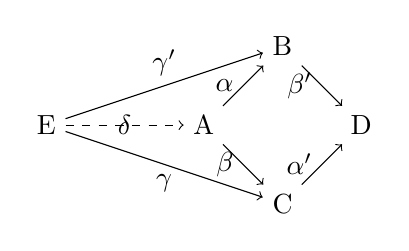
\begin{tikzpicture}
                        \node (i) at (0,0) {A};
                        \node (r) at (1,1) {B};
                        \node (c) at (1,-1) {C};
                        \node (h) at (2,0) {D}; 
                        % \node () at (1,-1) {\( \Delta \)};
                        \draw[->]  (i) -- (r) node [midway,left] {$\alpha$};
                        \draw[->] (c) -- (h) node [midway,left] {$\alpha'$};
                        \draw[->] (r) -- (h) node[midway, left] {$\beta'$};
                        \draw[->] (i) -- (c) node[midway, left] {$\beta$};
                        \node (d') at (-2,0) {E};
                        \draw[<-] (c) -- (d') node [midway,below]{$\gamma$};
                        \draw[<-] (r) -- (d') node [midway,above]{$\gamma'$};
                        \draw[->, dashed] (d') -- (i) node [midway]{$\delta$};
                    \end{tikzpicture}
        }
    %     \caption{}
    %     \label{fig:preliminaries:pullback_ssdsfd}
    % \end{figure}
                \end{center}
The diagram involving \( (\alpha, \beta, \alpha', \beta') \) is called a \textbf{pullback square}, or simply a \textbf{pullback}\index{Pullback!square}, with \(A\) as the \textbf{pullback object}\index{Pullback!object}. The existence of a unique morphism is known as the \textbf{universal mapping property of the pullback}\index{Pullback!universal mapping property}.
\end{definition} 

\begin{example} 
    \label{ex:cat:pbfsdljkgjasssss}
    In the category \textbf{Set},
    the pullback 
    of a cospan \(B \overset{\beta'}{\rightarrow} D \overset{\alpha'}{\leftarrow} C \) is the span \( B \overset{\alpha}{\leftarrow} A \overset{\beta}{\rightarrow} C \) where
    the pullback object is the set $A \mathop{=} \set{(b,c)\in B \mathop{\times} C \mathop{\mid} \beta (c) \mathop{=} \alpha (b)}$; $\alpha$ and $\beta$ are defined as the corresponding projections, e.g., $\alpha((b, c)) \mathop{=} b$ and $\beta((b, c)) \mathop{=} c$.
    Consider the following diagram in the category \textbf{Set}, where 
    sets are drawn as boxes,
    circles represent elements of sets, and numbers inside circles indicate how the functions map those elements.
    \begin{center}
      \resizebox{0.7\textwidth}{!}{
      \begin{tikzpicture}
          \graphbox{\( A\)}{40mm}{-3mm}{34mm}{12mm}{2mm}{2mm}{
              \coordinate (o) at (0mm,-8mm); 
              \node[draw,circle] (l1) at ($(o)+(-10mm,0mm)$) {1};
              \node[draw,circle] (l2) at ($(l1)+(2,0)$) {2};
          }  
          \graphbox{\( B \)}{80mm}{-3mm}{45mm}{12mm}{2mm}{2mm}{
              \coordinate (o) at (-5mm,-8mm); 
              \node[draw,circle] (l1) at ($(o)+(-10mm,0mm)$) {1};
              \node[draw,circle] (l2) at ($(l1)+(3,0)$) {2};
              \node[draw,circle] (l3) at ($(l1)+(1,0)$) {4};
            %   \node[draw,circle] (l4) at ($(l1)+(2,0)$) {5};
            %   \draw[ ] (l1) -- (l3) node[midway,above] {$a$};
            %   \draw[ ] (l3) -- (l4) node[midway,above] {$b$};
            %   \draw[ ] (l4) -- (l2) node[midway,above] {$a$};
          }     
          \graphbox{\( C  \)}{40mm}{-22mm}{34mm}{22mm}{2mm}{-3mm}{
              \coordinate (o) at (0mm,-3mm); 
              \node[draw,circle] (l1) at ($(o)+(-10mm,0mm)$) {1};
              \node[draw,circle] (l2) at ($(l1)+(2,0)$) {2};
            %   \node[draw,circle] (l4) at ($(l2)+(0,-1)$) {6};
              \node[ draw,circle] (l6) at ($(l1)+(0,-1)$) {3};
            %   \draw[ ] (l1) -- (l6) node[midway,left] {$a$};
            %   \draw[ ] (l2) -- (l4) node[midway,right] {$a$};
          }    
          \graphbox{\( D \)}{80mm}{-22mm}{45mm}{22mm}{2mm}{-3mm}{
              \coordinate (o) at (-5mm,-3mm); 
              \node[draw,circle] (l1) at ($(o)+(-10mm,0mm)$) {1};
              \node[draw,circle] (l2) at ($(l1)+(3,0)$) {2};
              \node[draw,circle] (l3) at ($(l1)+(1,0)$) {4};
            %   \node[draw,circle] (l4) at ($(l1)+(2,0)$) {5};
            %   \node[ draw,circle] (l5) at ($(l2)+(0,-1)$) {6};
              \node[ draw,circle] (l6) at ($(l1)+(0,-1)$) {3};
            %   \draw[ ] (l1) -- (l6) node[midway,left] {$a$};
            %   \draw[] (l1) -- (l3) node[midway,above] {$a$};
            %   \draw[] (l3) -- (l4) node[midway,above] {$b$};
            %   \draw[ ] (l4) -- (l2) node[midway,above] {$a$};
            %   \draw[ ] (l2) -- (l5) node[midway,right] {$a$};
          }    
          \node () at (77mm,-8mm) {\( \overset{\alpha}{\rightarrow} \)};
          \node () at (58mm,-18mm) {\( \beta\downarrow \)};
          \node () at (102mm,-18mm) {\( \beta'\downarrow \)};
          \node () at (77mm,-33mm) {\( \overset{\alpha'}{\rightarrow} \)};
      \end{tikzpicture}
      }
    \end{center} 
    The span \( B \overset{\alpha}{\leftarrow} A \overset{\beta}{\rightarrow} C \)
    % shown in Figure~\ref{fig:preliminaries:a_rewriting_step_dfjalsdkdfsdfjflg} 
    is the pullback of the cospan \(B \overset{\beta'}{\rightarrow} D \overset{\alpha'}{\leftarrow} C \).
    Indeed, the pullback object can be taken as the set $A' \mathop{=} \set{(1_B,1_C),(2_B,2_C)} \mathop{\subseteq} B \mathop{\times} C$, and the morphisms $\alpha'' \mathop{\colon} A'  \mathop{\to} B$ and $\beta'' \mathop{\colon} A'  \mathop{\to} C$ are defined as the corresponding projections, e.g., $\alpha''((x,y)) \mathop{=} x$ and $\beta''((x,y)) \mathop{=} y$. Note that $A$ is isomorphic to $A'$, which is expected because the pullback of a cospan is unique up to isomorphism.
\end{example}
In the category \textbf{Graph} pullbacks always exist and are computed pointwise: take the pullback in \textbf{Set} of the node sets and of the edge sets, and equip the resulting graph with source, target and labeling maps induced componentwise; the projection graph homomorphisms are the corresponding componentwise projections and they satisfy the universal property.
\begin{example}
    \label{ex:cat:pbfsdljkgjasssss2222ssss}
    Consider the diagram in the category \textbf{Graph}, shown below. The numbers inside nodes and the subgraphs in different colors illustrate how the morphisms map nodes and edges. 
    The span $L \overset{\alpha}{\leftarrow} K \overset{\beta}{\rightarrow} C$ is a pullback of the cospan $L \overset{\beta'}{\rightarrow} G \overset{\alpha'}{\leftarrow} C$.
    % \begin{figure}[H]
    %     \centering
    \begin{center}
        \resizebox{0.8\textwidth}{!}{
        \begin{tikzpicture} 
            \graphbox{\( L \)}{40mm}{20mm}{34mm}{20mm}{2mm}{2mm}{
                \coordinate (o) at (0mm,-10mm); 
                \node[draw,circle] (l1) at ($(o)+(-10mm,0mm)$) {1};
                \node[draw,circle] (l2) at ($(l1)+(2,0)$) {2};
                \draw[->,red] (l2) edge[out=-135,in=-45]node[midway,below] {$a$} (l1) ;
                \node[draw,circle,red] (l3) at ($(l1)+(1,0)$) {3};
                \draw[->,red] (l1) -- (l3) node[midway,above] {$a$};
                \draw[->,red] (l3) -- (l2) node[midway,above] {$a$};
            } 
    
            \graphbox{\( K \)}{0mm}{0mm}{34mm}{12mm}{2mm}{2mm}{
                \coordinate (o) at (0mm,-8mm); 
                \node[draw,circle] (l1) at ($(o)+(-10mm,0mm)$) {1};
                \node[draw,circle] (l2) at ($(l1)+(2,0)$) {2};
            }  
            \graphbox{\(G  \)}{90mm}{10mm}{34mm}{40mm}{2mm}{-3mm}{
                \coordinate (o) at (0mm,-20mm); 
                 \node[draw,circle] (l1) at ($(o)+(0,0)$) {1\ 2};
                % \node[draw,circle] (l1) at ($(o)+(-10mm,0mm)$) {1};
                % \node[draw,circle] (l2) at ($(l1)+(2,0)$) {2};
                \draw[->,red] (l1) edge[loop below] node[midway, below] {$a$} (l1) ;
                \node[draw,circle,red] (l3) at ($(l1)+(0,1.4)$) {3};
                \node[draw,circle,blue] (l4) at ($(l1)+(1,-1)$) {6};
                \draw[->,red] (l1) edge[bend left] node[midway,left] {$a$} (l3);
                \draw[->,red] (l3) edge[bend left] node[midway,right] {$a$} (l1);
                \draw[->,blue] (l1) edge  node[midway,right] {$a$} (l4);
                \node[draw,circle,blue] (l6) at ($(l1)+(-1,-1)$) {7};
                \draw[<-,blue] (l1) edge node[midway,left] {$a$} (l6) ;
                % \draw[->,blue] (l1) edge[out=-135,in=-45]node[midway,below] {$a$} (l1) ;
            }   
     
            \graphbox{\( C \)}{40mm}{-12mm}{34mm}{24mm}{2mm}{-3mm}{
                \coordinate (o) at (0mm,-5mm); 
                \node[draw,circle] (l1) at ($(o)+(0,0)$) {1\ 2};
                % \node[draw,circle] (l2) at ($(l1)+(2,0)$) {2};
                \node[draw,circle,blue] (l4) at ($(l1)+(1,-1)$) {6};
                \draw[->,blue] (l1) -- (l4) node[midway,right] {$a$};
                % \draw[->,blue] (l1) edge[loop above] node[midway, above] {$a$} (l1) ;
                \node[ draw,circle,blue] (l6) at ($(l1)+(-1,-1)$) {7};
                \draw[<-,blue] (l1) -- (l6) node[midway,left] {$a$};
            }
            % K to L  
            \draw[>->] (17mm,5mm) -- node[above] {$\alpha$} (37mm,15mm);
            % C to G
            \draw[>->] (76mm,-28mm)-- node[below] {$\alpha'$} (88mm,-26mm) ;
            % K to C
            \draw[->] (17mm,-17mm) -- node[below] {$\beta$} (37mm,-28mm);
            % L to G 
            \draw[->] (76mm,16mm) -- node[above] {$\beta'$} (88mm,10mm);
            \node () at (57mm,-6mm) {$PB$};
        \end{tikzpicture}
        }
    \end{center}
\end{example} 
Consider the following diagram in the category \textbf{Graph}:\begin{center}
        \resizebox{0.8\textwidth}{!}{
        \begin{tikzpicture} 
            \graphbox{\( L \)}{40mm}{15mm}{34mm}{12mm}{2mm}{2mm}{
                \coordinate (o) at (0mm,-8mm); 
                \node[draw,circle] (l1) at ($(o)+(-10mm,0mm)$) {1};
                \node[draw,circle] (l2) at ($(l1)+(2,0)$) {2};
                \node[draw,circle,red] (l3) at ($(l1)+(1,0)$) {3};
                \draw[->,red] (l1) -- (l3) node[midway,above] {$a$};
                \draw[->,red] (l3) -- (l2) node[midway,above] {$a$};
            } 
    
            \graphbox{\( K \)}{0mm}{0mm}{34mm}{12mm}{2mm}{2mm}{
                \coordinate (o) at (0mm,-8mm); 
                \node[draw,circle] (l1) at ($(o)+(-10mm,0mm)$) {1};
                \node[draw,circle] (l2) at ($(l1)+(2,0)$) {2};
            }  
            \graphbox{\(G  \)}{90mm}{5mm}{34mm}{24mm}{2mm}{-3mm}{
                \coordinate (o) at (0mm,-5mm); 
                \node[draw,circle] (l1) at ($(o)+(-10mm,0mm)$) {1};
                \node[draw,circle] (l2) at ($(l1)+(2,0)$) {2};
                \node[draw,circle,red] (l3) at ($(l1)+(1,0)$) {3};
                \node[draw,circle,blue] (l4) at ($(l2)+(0,-1)$) {6};
                \draw[->,red] (l1) -- (l3) node[midway,above] {$a$};
                \draw[->,red] (l3) -- (l2) node[midway,above] {$a$};
                \draw[->,blue] (l2) -- (l4) node[midway,right] {$a$};
                \node[draw,circle,blue] (l6) at ($(l1)+(0,-1)$) {7};
                \draw[<-,blue] (l1) -- (l6) node[midway,left] {$a$};
                \draw[->,blue] (l2) edge[out=-135,in=-45]node[midway,below] {$a$} (l1) ;
            }   
     
            \graphbox{\( C \)}{40mm}{-15mm}{34mm}{24mm}{2mm}{-3mm}{
                \coordinate (o) at (0mm,-5mm); 
                \node[draw,circle] (l1) at ($(o)+(-10mm,0mm)$) {1};
                \node[draw,circle] (l2) at ($(l1)+(2,0)$) {2};
                \node[draw,circle,blue] (l4) at ($(l2)+(0,-1)$) {6};
                \draw[->,blue] (l2) -- (l4) node[midway,right] {$a$};
                \draw[->,blue] (l2) edge[out=-135,in=-45]node[midway,below] {$a$} (l1) ;
                \node[ draw,circle,blue] (l6) at ($(l1)+(0,-1)$) {7};
                \draw[<-,blue] (l1) -- (l6) node[midway,left] {$a$};
            }      
            % K to L
            \draw[>->] (17mm,5mm) -- node[above] {$\alpha$} (37mm,10mm);
            % C to G
            \draw[>->] (76mm,-28mm)-- node[below] {$\alpha'$} (104mm,-21mm) ;
            % K to C
            \draw[>->] (17mm,-17mm) -- node[below] {$\beta$} (37mm,-28mm);
            % L to G
            \draw[>->] (76mm,10mm) -- node[above] {$\beta'$} (104mm,7mm);
            \node () at (57mm,-6mm) {$PO$};
        \end{tikzpicture}
        }
    \end{center}
We observe that it is a pushout square as well as a pullback square. This is not a coincidence, as stated in the following proposition.
\begin{proposition}[\text{\cite[Lemma 13]{lack2004adhesive}}]
    \label{prop:pb_eq_po}
    In the category \textbf{Graph}, pushouts along monomorphisms are also pullbacks. 
\end{proposition}
This proposition is illustrated in Example~\ref{ex:cat:pushout_non_injective_ssss} and Example~\ref{ex:cat:pbfsdljkgjasssss2222ssss}.


\begin{notation}
    When the context makes it clear, a morphism \( h : A \to B \) will be denoted by \( h_{AB} \), and diagrams will be referred to by their nodes, as is standard in geometry. For example, the diagram involving the morphisms \( \alpha, \beta, \alpha', \beta' \) in~\autoref{def:cat:po} will be denoted by \( ACDB \) or \( ABDC \).
\end{notation}   

\subsection{DPO rewriting}
\label{preliminaries:grs}
\begin{definition}[Rewriting rule and match~\cite{corradini1997algebraic}]
  \label{def:grs:dpo_rule}
A \textbf{DPO rewriting rule} $\rho$ is a span \( L \overset{l}{\leftarrow} K \overset{r}{\rightarrow} R \), where \( K \) is the \textbf{interface}, \( L \) is the \textbf{left-hand-side graph}, denoted \( \operatorname{lhs}(\rho) \), and \( R \) is the \textbf{right-hand-side graph}, denoted \( \operatorname{rhs}(\rho) \). The rule is \textbf{monic} if $l$ and $r$ are both monic.
A match of the rule in an graph \( G \) is a morphism \( m: L \rightarrow G \).   
\end{definition}
   In this paper, we use examples from the category \textbf{Graph} of edge-labeled directed multigraphs (see~\cite{konig2018atutorial}) to illustrate the discussed concepts. To facilitate this, we introduce the following notation for visualizing graph homomorphisms.
\begin{notation}[\cite{qiu2025termination}]
    We use the notation from~\cite[Notation 1]{overbeek2023apbpotutorial} to visualize edge-labeled graph homomorphisms. Labeled graphs are enclosed in boxes with their names displayed in the top-left corner. Nodes and edges are assigned subsets of \(\mathbb{N}\) as identifiers, and these identifiers are chosen such that: (i) Each node or edge \( y \) in the codomain graph is assigned the union of the identifiers of all nodes or edges in the domain graph that are mapped to \( y \); (ii) The graph homomorphism is uniquely determined by this assignment. To further improve readability, we represent sets by listing their elements. Additionally, we omit identifiers when doing so does not cause confusion. This is illustrated in the following representation of a homomorphism \( h: G \to H \).
    
   \begin{center}
        \resizebox{0.5\textwidth}{!}{
        \begin{tikzpicture}
            \graphbox{\( G \)}{00mm}{-20mm}{45mm}{25mm}{2mm}{-10mm}{
                \coordinate (o) at (-5mm,-8mm); 
                \node[draw,circle] (l1) at ($(o)+(-10mm,0mm)$) {1};
                \node[draw,circle] (l2) at ($(l1)+(3,0)$) {2};
                \node[draw,circle] (l3) at ($(l1)+(1,0)$) {3};
                \node[draw,circle] (l4) at ($(l1)+(2,0)$) {4};
                \draw[->] (l1) -- (l3) node[midway,above] {a};
                \draw[->] (l3) -- (l4) node[midway,above] {b};
                \draw[->] (l4) -- (l2) node[midway,above] {a};
            }  
            \graphbox{\( H \)}{52mm}{-20mm}{50mm}{25mm}{2mm}{-10mm}{
                \coordinate (o) at (-5mm,-8mm); 
                \node[draw,circle] (l1) at ($(o)+(-1,0mm)$) {1};
                \node[draw,circle] (l2) at ($(l1)+(3,0)$) {2};
                \node[draw,circle] (l3) at ($(l1)+(1.5,0)$) {3\ 4};
                \draw[->] (l1) edge node[midway,above] {a} (l3);
                \draw[->] (l3) edge [loop above] node[midway,above] {b} (l3) ;
                \draw[->] (l3) -- (l2) node[midway,above] {a};
            }      
            \node () at (48mm,-30mm) {$\rightarrow$};
        \end{tikzpicture}
    }
    \end{center}  
    In this example, the sets \(\{1\}\), \(\{2\}\), \(\{3\}\), \(\{4\}\), and \(\{3,4\}\) are represented as \(1\), \(2\), \(3\), \(4\), and \(3\ 4\), respectively. Edge identifiers are omitted.
\end{notation}
\begin{example}
  \label{ex:grsaa}
  The injective DPO rule from \cite[Example 6]{bruggink2014termination} will be used to illustrate the concepts discussed throughout this paper.
  The rule can be visualized as follows:
  \begin{center} 
      \resizebox{0.7\textwidth}{!}{
      \begin{tikzpicture}
          \graphbox{$L$}{0mm}{0mm}{34mm}{15mm}{2mm}{-5mm}{
              \coordinate (o) at (0mm,-3mm); 
              \node[draw,circle] (l1) at ($(o)+(-10mm,0mm)$) {1};
              \node[draw,circle] (l2) at ($(l1)+(2,0)$) {2};
              \node[draw,circle] (l3) at ($(l1) + (1,0)$) {3};
              \draw[->] (l1) -- (l3) node[midway,above] {a};
              \draw[->] (l3) -- (l2) node[midway,above] {a};
          }     
          \graphbox{$K$}{40mm}{0mm}{24mm}{15mm}{2mm}{-5mm}{
              \coordinate (o) at (5mm,-3mm); 
              \node[draw,circle] (l1) at ($(o)+(-10mm,0mm)$) {1};
              \node[draw,circle] (l2) at ($(l1)+(1,0)$) {2};
              % \node[draw,circle] (l3) at ($(l1) + (1,0)$) {$\ $};
              % \draw[->] (l1) -- (l3) node[midway,above] {a};
              % \draw[->] (l3) -- (l2) node[midway,above] {a};
          }    
          \graphbox{$R$}{70mm}{0mm}{45mm}{15mm}{2mm}{-5mm}{
              \coordinate (o) at (-5mm,-3mm); 
              \node[draw,circle] (l1) at ($(o)+(-10mm,0mm)$) {1};
              \node[draw,circle] (l2) at ($(l1)+(3,0)$) {2};
              \node[draw,circle] (l3) at ($(l1) + (1,0)$) {4};
              \node[draw,circle] (l4) at ($(l1) + (2,0)$) {5};
              \draw[->] (l1) -- (l3) node[midway,above] {a};
              \draw[->] (l3) -- (l4) node[midway,above] {b};
              \draw[->] (l4) -- (l2) node[midway,above] {a};
          }    
          \node () at (37mm,-8mm) {$\overset{l}{\leftarrowtail}$};
          \node () at (67mm,-8mm) {$\overset{r}{\rightarrowtail}$};
          % \draw[>->] (51mm,2mm) -- (52mm,3mm);
      \end{tikzpicture}
      }
  \end{center}
\end{example}
\begin{definition}[DPO Rewriting step \cite{endrullis2024generalized_arxiv_v2}]
  \label{def:rewriting_step}
    \ \newline
    \noindent
    \begin{minipage}{0.72\textwidth}
      A DPO diagram $\delta$ is a diagram as shown on the right.
      This diagram $\delta$ is a witness for the \textbf{rewriting step} from \( G \) to \( H \) using the rule \( \rho \) and \textbf{match} \( m \), denoted \( G \mathop{\Rightarrow}_\rho^m H \) or \( G \mathop{\Rightarrow}_\rho^\delta H \). We denote $\operatorname{left}(\delta)$ and $\operatorname{right}(\delta)$ the pushout squares $KLGC$ and $KRHC$, respectively.
    \end{minipage}
    \hfill
    \begin{minipage}{0.28\textwidth}
          % \begin{center}
          \hfill
          \resizebox{0.85\textwidth}{!}{
          \begin{tikzpicture}
            % [node distance=11mm]
            \node (I) at (0,0) {$K$};
            \node (L) at (-2,0) {$L$};
            \node (R) at (2,0) {$R$};
            \node (G) at (-2,-2) {$G$};
            \node (C) at (0,-2) {$C$};
            \node (H) at (2,-2) {$H$};
            \draw [->] (I) to  node [midway,below] {$l$} (L);
            \draw [->] (I) to  node [midway,below] {$r$} (R);
            \draw [->] (L) to node [midway,right] {$m$} (G);
            \draw [->] (I) to node [midway,right] {$u$} (C);
            \draw [->] (R) to node [midway,left] {$m'$} (H);
            \draw [->] (C) to node [midway,above] {$l'$} (G);
            \draw [->] (C) to node [midway,above] {$r'$} (H);
            \node [at=($(I)!.5!(G)$)] {\normalfont PO};
            \node [at=($(I)!.5!(H)$)] {\normalfont PO};
          \end{tikzpicture}
        % \end{center}
        }
        \end{minipage}
  \end{definition}
\begin{example}
  \label{ex:rewriting_step_grs_aa}
  The DPO diagram below defines a rewriting step using the rule from Example~\ref{ex:grsaa}.
  \begin{center} 
      \resizebox{0.7\textwidth}{!}{
      \begin{tikzpicture}
          \graphbox{\( L \)}{0mm}{-3mm}{34mm}{12mm}{2mm}{2mm}{
              \coordinate (o) at (0mm,-8mm); 
              \node[draw,circle] (l1) at ($(o)+(-10mm,0mm)$) {1};
              \node[draw,circle] (l2) at ($(l1)+(2,0)$) {2};
              \node[draw,circle] (l3) at ($(l1)+(1,0)$) {3};
              \draw[] (l1) -- (l3) node[midway,above] {$a$};
              \draw[] (l3) -- (l2) node[midway,above] {$a$};
          } 
          \graphbox{\( K \)}{40mm}{-3mm}{34mm}{12mm}{2mm}{2mm}{
              \coordinate (o) at (0mm,-8mm); 
              \node[draw,circle] (l1) at ($(o)+(-10mm,0mm)$) {1};
              \node[draw,circle] (l2) at ($(l1)+(2,0)$) {2};
          }  
          \graphbox{\( R \)}{80mm}{-3mm}{45mm}{12mm}{2mm}{2mm}{
              \coordinate (o) at (-5mm,-8mm); 
              \node[draw,circle] (l1) at ($(o)+(-10mm,0mm)$) {1};
              \node[draw,circle] (l2) at ($(l1)+(3,0)$) {2};
              \node[draw,circle] (l3) at ($(l1)+(1,0)$) {4};
              \node[draw,circle] (l4) at ($(l1)+(2,0)$) {5};
              \draw[ ] (l1) -- (l3) node[midway,above] {$a$};
              \draw[ ] (l3) -- (l4) node[midway,above] {$b$};
              \draw[ ] (l4) -- (l2) node[midway,above] {$a$};
          }    
          \graphbox{\( G \)}{0mm}{-22mm}{34mm}{22mm}{2mm}{-3mm}{
              \coordinate (o) at (0mm,-3mm); 
              \node[draw,circle] (l1) at ($(o)+(-10mm,0mm)$) {1};
              \node[draw,circle] (l2) at ($(l1)+(2,0)$) {2};
              \node[draw,circle] (l3) at ($(l1)+(1,0)$) {3};
              \node[draw,circle] (l4) at ($(l2)+(0,-1)$) {6};
              \draw[] (l1) -- (l3) node[midway,above] {$a$};
              \draw[] (l3) -- (l2) node[midway,above] {$a$};
              \draw[ ] (l2) -- (l4) node[midway,right] {$a$};
              \node[draw,circle] (l6) at ($(l1)+(0,-1)$) {7};
              \draw[] (l1) -- (l6) node[midway,left] {$a$};
          }    
          \graphbox{\( C  \)}{40mm}{-22mm}{34mm}{22mm}{2mm}{-3mm}{
              \coordinate (o) at (0mm,-3mm); 
              \node[draw,circle] (l1) at ($(o)+(-10mm,0mm)$) {1};
              \node[draw,circle] (l2) at ($(l1)+(2,0)$) {2};
              \node[draw,circle] (l4) at ($(l2)+(0,-1)$) {6};
              \draw[ ] (l2) -- (l4) node[midway,right] {$a$};
              \node[ draw,circle] (l6) at ($(l1)+(0,-1)$) {7};
              \draw[ ] (l1) -- (l6) node[midway,left] {$a$};
          }    
          \graphbox{\( H \)}{80mm}{-22mm}{45mm}{22mm}{2mm}{-3mm}{
              \coordinate (o) at (-5mm,-3mm); 
              \node[draw,circle] (l1) at ($(o)+(-10mm,0mm)$) {1};
              \node[draw,circle] (l2) at ($(l1)+(3,0)$) {2};
              \node[draw,circle] (l3) at ($(l1)+(1,0)$) {4};
              \node[draw,circle] (l4) at ($(l1)+(2,0)$) {5};
              \node[ draw,circle] (l5) at ($(l2)+(0,-1)$) {6};
              \node[ draw,circle] (l6) at ($(l1)+(0,-1)$) {7};
              \draw[ ] (l1) -- (l6) node[midway,left] {$a$};
              \draw[] (l1) -- (l3) node[midway,above] {$a$};
              \draw[] (l3) -- (l4) node[midway,above] {$b$};
              \draw[ ] (l4) -- (l2) node[midway,above] {$a$};
              \draw[ ] (l2) -- (l5) node[midway,right] {$a$};
          }    
          \node () at (37mm,-8mm) {\( \leftarrowtail \)}; % K -> L
          \node () at (77mm,-8mm) {\( \rightarrowtail \)}; % K -> R
          \node () at (15mm,-18mm) {\( m\ \downarrowtail \)};
          \node () at (37mm,-33mm) {\( \leftarrowtail \)};
          \node () at (58mm,-18mm) {\( u\downarrowtail \)};
          \node () at (102mm,-18mm) {\( \downarrowtail \)};
          \node () at (77mm,-33mm) {\( \rightarrowtail \)}; % C -> H
      \end{tikzpicture}
      }
  \end{center}
\end{example}
DPO rewriting has several variants, depending on factors such as whether the matching morphism, the left-hand morphism, or the right-hand morphism is monic~\cite{habel2001double}, and whether the left pushout square is restricted~\cite{behr2021concurrency,behr2023fundamentals}. Since these restrictions can influence the termination properties of a DPO rewrite system,  we use the parametric definition presented in~\cite{EndrullisOverbeek2024Generalized} to encompass different DPO variants.
% \begin{definition}[DPO rewriting framework~\cite{endrullis2024generalized_arxiv_v2}]
%     A \emph{DPO rewriting framework} $\mathfrak{F}$ is a mapping of DPO rewriting rules to classes of DPO diagrams such that, for every DPO rule $\rho$, $\mathfrak{F}(\rho)$ is a class of DPO diagrams with top-span $\rho$.
    
%     The DPO rewriting relation $\Rightarrow_{\rho,\mathfrak{F}}$ induced by a DPO rewriting rule $\rho$ in $\mathfrak{F}$ is defined as follows: $G \Rightarrow_{\rho,\mathfrak{F}} H$ iff $G \Rightarrow_\rho^\delta H$ for some $\delta \in \mathfrak{F}(\rho)$. 
%     % for some $\delta \in \mathfrak{F}(\rho)$
%     The rewriting relation $\Rightarrow_{\mathcal{R},\mathfrak{F}}$ induced by a set $\mathcal{R}$ of DPO rewriting rules in $\mathfrak{F}$ is given by: $G \Rightarrow_{\mathcal{R},\mathfrak{F}} H$ iff $G \Rightarrow_{\rho,\mathfrak{F}} H$ for some $\rho \in \mathcal{R}$. When $\mathfrak{F}$ is clear from the context, we 
%     suppress $\mathfrak{F}$ and 
%     write $\Rightarrow_{\rho}$ and $\Rightarrow_{\mathcal{R}}$.
% \end{definition} 
\begin{definition}[Rewriting framework~\cite{endrullis2024generalized_arxiv_v2}]
    A \textbf{DPO rewriting framework} $\mathfrak{F}$ is a mapping of DPO rewriting rules to collections of DPO diagrams. Specifically, for every rule \( \rho = (L \overset{l}{\leftarrow} K \overset{r}{\rightarrow} R) \), the collection $\mathfrak{F}(\rho)$ consists of DPO diagrams of the form shown in Definition~\ref{def:rewriting_step}.

    The \textbf{DPO rewriting relation $\Rightarrow_{\rho,\mathfrak{F}}$ induced by a DPO rewriting rule $\rho$ in $\mathfrak{F}$} is defined as follows: $G \Rightarrow_{\rho,\mathfrak{F}} H$ iff $G \Rightarrow_\rho^\delta H$ for some $\delta \in \mathfrak{F}(\rho)$. 
    % for some $\delta \in \mathfrak{F}(\rho)$
     The \textbf{DPO rewriting relation $\Rightarrow_{\mathcal{R},\mathfrak{F}}$ induced by a set $\mathcal{R}$ of DPO rewriting rules in $\mathfrak{F}$} is given by: $G \Rightarrow_{\mathcal{R},\mathfrak{F}} H$ iff $G \Rightarrow_{\rho,\mathfrak{F}} H$ for some $\rho \in \mathcal{R}$. When $\mathfrak{F}$ is clear from the context, we 
    suppress $\mathfrak{F}$ and 
    write $\Rightarrow_{\rho}$ and $\Rightarrow_{\mathcal{R}}$.
  \end{definition}
\subsection{Relative termination}
  \label{preliminaries:relative_termination}
\begin{definition}[Rewriting sequence]
    Let \(\mathcal{R}\) be a set of rewriting rules. Let $\mathfrak{F}$ be a DPO rewriting framework.
    A \textbf{$(\mathcal{R},\mathfrak{F})$-rewriting sequence} is a finite sequence \(s_0,s_1,\hdots, s_m\) of objects such that \(s_n \Rightarrow_{\mathcal{R},\mathfrak{F}} s_{n+1}\) for each \( 0 \leq n \leq m-1\), or an infinite sequence \(s_0,s_1,\hdots\) of objects such that \(s_n \Rightarrow_{\mathcal{R},\mathfrak{F}} s_{n+1}\) for each \(n \in \mathbb{N}\).
    A $(\mathcal{R},\mathfrak{F})$-rewriting sequence from \( s_0 \) will be denoted as:
    \(
    s_0 \Rightarrow_{\mathcal{R},\mathfrak{F}} s_1 \Rightarrow_{\mathcal{R},\mathfrak{F}} s_2 \Rightarrow_{\mathcal{R},\mathfrak{F}} \cdots 
    \)
\end{definition}
% \todo{plus generalement, c'est defini sur des relations, pas forcement de reecriture}
% \begin{definition} 
%     Let \(\mathcal{R}\) be a set of rewriting rules and let $\mathfrak{F}$ be a DPO rewriting framework.
%     An \textbf{$(\mathcal{R},\mathfrak{F})$-rewriting sequence} is either  
%     \begin{itemize}
%         \item a finite sequence \(s_0,s_1,\hdots, s_m\) of objects such that \( s_n \Rightarrow_{\mathcal{R},\mathfrak{F}} s_{n+1}\text{ for each } 0 \leq n \leq m-1\), or
%         \item an infinite sequence \(s_0,s_1,\hdots\) of objects such that \(s_n \Rightarrow_{\mathcal{R},\mathfrak{F}} s_{n+1}\) for each \(n \in \mathbb{N}\).
%     \end{itemize}
%     An $(\mathcal{R},\mathfrak{F})$-rewriting sequence from \( s_0 \) will be denoted by:
%     \[
%     s_0 \Rightarrow_{\mathcal{R},\mathfrak{F}} s_1 \Rightarrow_{\mathcal{R},\mathfrak{F}} s_2 \Rightarrow_{\mathcal{R},\mathfrak{F}} \cdots 
%     \]
% \end{definition}
Given a DPO rewriting framework \(\mathfrak{F}\), a rule set \(\mathcal{R}\) defines the binary relation \enquote{object $X$ can be rewritten to object $Y$ using rules from the rule set} on the objects of the category $\mathcal{C}$.
\begin{definition}\label{def:rewriting-chain}
Let \(\mathcal{R}\) be a rule set and let \(\mathfrak{F}\) be a DPO rewriting framework.
An \textbf{\((\mathcal{R},\mathfrak{F})\)-rewriting chain} is a \(\Rightarrow_{\mathcal{R},\mathfrak{F}}\)-chain. Hence, when the context is clear, we simply call it a \textbf{rewriting chain}.
\end{definition}

\begin{example}
    Consider the rewriting rules in~\autoref{fig:preliminaries:graph_transformation_rule_nonterminating}, which
    replaces an occurrence of the graph 
\raisebox{2pt}{
            \scalebox{0.7}{\tikz[baseline=-0.5ex]{
            \node [draw,circle] (z) at (-1,0) {};
            \node [draw,circle] (x) at (0,0) {};
            \node[draw,circle] (y) at (1,0) {};
            \draw[->] (z)--(x) node[midway, above] {$a$};
            \draw[->] (x)--(y) node[midway, above] {$b$};
        }}} with an occurrence of the graph \raisebox{2pt}{
            \scalebox{0.7}{\tikz[baseline=-0.5ex]{
            \node [draw,circle] (z) at (-1,0) {};
            \node [draw,circle] (x) at (0,0) {};
            \node[draw,circle] (y) at (1,0) {};
            \draw[->] (z)--(x) node[midway, above] {$b$};
            \draw[->] (x)--(y) node[midway, above] {$a$};
        }}}, keeping the extreme nodes unchanged.
    \begin{figure}[H]
        \centering
            \resizebox{0.85\textwidth}{!}{
                \begin{tikzpicture}[baseline=-3ex]
                    \graphbox{\( L \)}{0mm}{-3mm}{34mm}{15mm}{2mm}{2mm}{
                        \coordinate (o) at (0mm,-11mm); 
                        \node[draw,circle] (l1) at ($(o)+(-10mm,0mm)$) {1};
                        \node[draw,circle] (l2) at ($(l1)+(2,0)$) {2};
                        \node[draw,circle] (l3) at ($(l1) + (1,0)$) {3};
                        \draw[->] (l1) -- (l3) node[midway,above] {$a$};
                        \draw[->] (l3) -- (l2) node[midway,above] {$b$};
                    } 
            
                    \graphbox{\( K \)}{40mm}{-3mm}{34mm}{15mm}{2mm}{2mm}{
                        \coordinate (o) at (0mm,-11mm); 
                        \node[draw,circle] (l1) at ($(o)+(-10mm,0mm)$) {1};
                        \node[draw,circle] (l2) at ($(l1)+(2,0)$) {2};
                    }  
            
                    \graphbox{\( R \)}{80mm}{-3mm}{35mm}{15mm}{2mm}{2mm}{
                        \coordinate (o) at (-5mm,-11mm); 
                        \node[draw,circle] (l1) at ($(o)+(-10mm,0mm)$) {1};
                        % \node[draw,circle] (l2) at ($(l1)+(3,0)$) {2};
                        \node[draw,circle] (l3) at ($(l1) + (1,0)$) {4};
                        \node[draw,circle] (l4) at ($(l1) + (2,0)$) {2};
                        \draw[->] (l1) -- (l3) node[midway,above] {$b$};
                        \draw[->] (l3) -- (l4) node[midway,above] {$a$};
                        % \draw[->] (l4) -- (l2) node[midway,above] {$a$};
                    }    
                    \node () at (37mm,-10mm) {\( \leftarrowtail \)}; % K -> L
                    \node () at (77mm,-10mm) {\( \rightarrowtail \)}; % K -> R
                \end{tikzpicture}
                }
        \caption{}
        \label{fig:preliminaries:graph_transformation_rule_nonterminating}
    \end{figure} 
  
    A looping rewriting chain using this rule is shown in~\autoref{fig:preliminaries:sequence_of_transformation_infinite}, in which the subgraph to be replaced at each transformation step is highlighted in red.
       
        \begin{figure}[H]
           \centering
          \resizebox{0.85\textwidth}{!}{
            \tikz
            [baseline=-0.5ex]
            { 
                \node[draw,circle] (x) at (0,0) {};
                \node[draw,circle] (y) at (1,0) {};
                \node[draw,circle] (z) at (0.5,0.86) {};
                \draw[->,red] (x) -- node[midway,below] {$a$} (y) ;
                \draw[->,red] (y) -- node[midway,right] {$b$} (z) ;
                \draw[->] (z) -- node[midway,left] {$b$} (x) ;
            } 
            $\Rightarrow$ 
            \tikz[baseline=-0.5ex]{ 
                \node[draw,circle] (x) at (0,0) {};  
                \node[draw,circle] (y) at (1,0) {};
                \node[draw,circle] (z) at (0.5,0.86) {};
                \draw[->] (x) -- node[midway,below] {$b$} (y) ;
                \draw[->,red] (y) -- node[midway,right] {$a$} (z) ;
                \draw[->,red] (z) -- node[midway,left] {$b$} (x) ;
            }
            $\Rightarrow$ 
            \tikz[baseline=-0.5ex]{ 
                \node[draw,circle] (x) at (0,0) {};  
                \node[draw,circle] (y) at (1,0) {};
                \node[draw,circle] (z) at (0.5,0.86) {};
                \draw[->,red] (x) -- node[midway,below] {$b$} (y) ;
                \draw[->] (y) -- node[midway,right] {$b$} (z) ;
                \draw[->,red] (z) -- node[midway,left] {$a$} (x) ;
            }
            $\Rightarrow$
            \tikz[baseline=-0.5ex]{ 
                \node[draw,circle] (x) at (0,0) {};   
                \node[draw,circle] (y) at (1,0) {};
                \node[draw,circle] (z) at (0.5,0.86) {};
                \draw[->,red] (x) -- node[midway,below] {$a$} (y) ;
                \draw[->,red] (y) -- node[midway,right] {$b$} (z) ;
                \draw[->] (z) -- node[midway,left] {$b$} (x) ;
            }
          }
          \caption{}
          \label{fig:preliminaries:sequence_of_transformation_infinite}
        \end{figure}
\end{example}

For a set of rewriting rules \(\mathcal{R}\) (and a DPO rewriting framework \(\mathfrak{F}\)), the impossibility of transforming any object infinitely with the non-deterministic strategy \enquote{apply rules as long as possible} using rules from \(\mathcal{R}\) (in the framework \(\mathfrak{F}\)) is called \emph{termination} in the literature~\cite{middeldorp1997simple}. This property corresponds to program termination on all inputs in conventional programming languages, and is undecidable in general~\cite{plump1998terminationundecidable}.

For example of a non-terminating rule set, consider the set with the unique rule shown in~\autoref{fig:preliminaries:graph_transformation_rule_nonterminating} and the infinite rewriting chain shown in~\autoref{fig:preliminaries:sequence_of_transformation_infinite}. 
For example of a terminating rule set, consider the set with the unique rule shown in~\autoref{fig:intro:edge_deletion_andffsfjsssdkdsglkadjl}, which deletes an edge. Any rewriting chain using this rule is finite, because each rewriting step decreases the number of edges by one and a graph has only finitely many edges by definition.
 \begin{figure}[H]
    \centering
     \resizebox{0.85\textwidth}{!}{ 
                \begin{tikzpicture}[baseline=-3ex]
                    \graphbox{\( L \)}{0mm}{-3mm}{34mm}{15mm}{2mm}{2mm}{
                        \coordinate (o) at (0mm,-11mm); 
                        \node[draw,circle] (l1) at ($(o)+(-10mm,0mm)$) {1};
                        \node[draw,circle] (l2) at ($(l1)+(2,0)$) {2};
                        % \node[draw,circle] (l3) at ($(l1) + (1,0)$) {3};
                        \draw[->] (l1) -- (l2) node[midway,above] {$a$};
                    } 
            
                    \graphbox{\( K \)}{40mm}{-3mm}{34mm}{15mm}{2mm}{2mm}{
                        \coordinate (o) at (0mm,-11mm); 
                        \node[draw,circle] (l1) at ($(o)+(-10mm,0mm)$) {1};
                        \node[draw,circle] (l2) at ($(l1)+(2,0)$) {2};
                    }  
            
                    \graphbox{\( R \)}{80mm}{-3mm}{35mm}{15mm}{2mm}{2mm}{
                        \coordinate (o) at (-5mm,-11mm); 
                        \node[draw,circle] (l1) at ($(o)+(-10mm,0mm)$) {1};
                        % \node[draw,circle] (l2) at ($(l1)+(3,0)$) {2};
                        % \node[draw,circle] (l3) at ($(l1) + (1,0)$) {4};
                        \node[draw,circle] (l4) at ($(l1) + (2,0)$) {2};
                        \draw[->] (l1) -- (l4) node[midway,above] {$b$};
                        % \draw[->] (l4) -- (l2) node[midway,above] {$a$};
                    }    
                    \node () at (37mm,-10mm) {\( \leftarrowtail \)}; % K -> L
                    \node () at (77mm,-10mm) {\( \rightarrowtail \)}; % K -> R
                \end{tikzpicture}
                }
                \caption{}
                \label{fig:intro:edge_deletion_andffsfjsssdkdsglkadjl}
        \end{figure}

However, in many cases, an interesting property can be proved even if the whole rule set is not terminating. For example, consider the graph transformation system with two rules shown in~\autoref{fig:intro:edge_deletion_and_node_addition_ruledfakdsjflsdaj}: rule $\alpha$ deletes an arbitrary edge labeled by $A$, and rule $\beta$ introduces a fresh node.
  \begin{figure}[H]
        \centering
%   \begin{subfigure}{0.3\textwidth}
%         % \centering
        $\alpha$ = {
             \resizebox{0.7\textwidth}{!}{
             \begin{tikzpicture}[baseline=-7ex]
                    \graphbox{\( \mathcal{L} \)}{0mm}{-3mm}{34mm}{15mm}{2mm}{2mm}{
                        \coordinate (o) at (0mm,-11mm); 
                        \node[draw,circle] (l1) at ($(o)+(-10mm,0mm)$) {$1$};
                        \node[draw,circle] (l2) at ($(l1)+(2,0)$) {$2$};
                        \draw[->] (l1) -- (l2) node[midway,above] {$A$};
                    } 
            
                    \graphbox{\( \mathcal{K} \)}{40mm}{-3mm}{34mm}{15mm}{2mm}{2mm}{
                        \coordinate (o) at (0mm,-11mm); 
                        \node[draw,circle] (l1) at ($(o)+(-10mm,0mm)$) {$1$};
                        \node[draw,circle] (l2) at ($(l1)+(2,0)$) {$2$};
                    }  
            
                    \graphbox{\( \mathcal{R} \)}{80mm}{-3mm}{35mm}{15mm}{5mm}{2mm}{
                        \coordinate (o) at (-5mm,-11mm); 
                        \node[draw,circle] (l1) at ($(o)+(-10mm,0mm)$) {$1$};
                        \node[draw,circle] (l4) at ($(l1) + (2,0)$) {$2$};
                    }    
                    \node () at (37mm,-10mm) {\( \leftarrowtail \)}; % K -> L
                    \node () at (77mm,-10mm) {\( \rightarrowtail \)}; % K -> R
                \end{tikzpicture}
            }
        }
    %     \caption{A graph transformation rule for edge deletion}
    % \label{fig:intro:edge_deletion_rule}
    % \end{subfigure}
    
    % \begin{subfigure}{0.3\textwidth}
    %     % \centering

        $\beta$ ={
             \resizebox{0.7\textwidth}{!}{
             \begin{tikzpicture}[baseline=-7ex]
                    \graphbox{\( \mathcal{L} \)}{0mm}{-3mm}{34mm}{15mm}{2mm}{2mm}{
                        
                    } 
            
                    \graphbox{\( \mathcal{K} \)}{40mm}{-3mm}{34mm}{15mm}{2mm}{2mm}{
                       
                    }  
            
                    \graphbox{\( \mathcal{R} \)}{80mm}{-3mm}{35mm}{15mm}{5mm}{2mm}{
                        \coordinate (o) at (0mm,-11mm); 
                        \node[draw,circle] (l1) at ($(o)+(-10mm,0mm)$) {};
                    }    
                    \node () at (37mm,-10mm) {\( \leftarrowtail \)}; % K -> L
                    \node () at (77mm,-10mm) {\( \rightarrowtail \)}; % K -> R
                \end{tikzpicture}
            }
        }
    %     \caption{A graph transformation rule for node addition}
    %     \label{fig:intro:node_addition_rule}
    % \end{subfigure} 
    \caption{}
    \label{fig:intro:edge_deletion_and_node_addition_ruledfakdsjflsdaj}
  \end{figure}
The system does not terminate because the node-adding rule $\beta$ can be applied indefinitely. However, the edge-deleting rule $\alpha$ can be applied a finite number of times only: it deletes an edge on each application, and since no rule increases the edge count and the initial graph is finite, only finitely many deletions are possible. Therefore, termination of the full system depends solely on the node-adding rule $\beta$. This observation motivates the more general property called \emph{relative termination}, which was originally introduced by Klop in~\cite{klop1987term} for binary relations, and has been studied and employed in the context of rewriting systems~\cite{geser1990relative,kassing2024dependency,endrullis2024generalized_icgt,zantema2014termination,bruggink2014termination,bruggink2015proving}. 

\begin{definition}
Let $A$ be a collection of objects and let $R$ and $S$ be binary relations on $A$. 
We say that $R$ is \textbf{terminating relative to} $S$ (or that $R$ \textbf{terminates relative to} $S$) if 
any $(R \cup S)$-chain contains only finitely many $R$-steps.
In particular, $R$ is \textbf{terminating} (or terminates) if it is terminating relative to the empty relation $\emptyset$.
\end{definition}

For example, the relation $>$ on $\mathbb{N}$ is terminating relative to the empty relation, since any $(> \cup \emptyset)$-chain contains only finitely many $>$-steps. The relation $>$ is also terminating relative to $\geq$ on $\mathbb{N}$, since any $(> \cup \geq)$-chain can only contain finitely many $>$-steps.

Note that termination and well-foundedness are the same property of a binary relation $\to$ described from two perspectives. Operationally, we read $x \to y$ as \enquote{$x$ can be transformed to $y$}; the absence of infinite $\rightarrow$-chains therefore means that any transformation sequence starting from an initial object $x$ is finite, i.e. every computation or rewrite sequence eventually terminates. Structurally, we read $x \to y$ as \enquote{$x$ is constructed from $y$}; the absence of infinite $\to$-chains then implies that every object $x$ can be traced back along a finite chain to an element that is not constructed from any other, so the structure is well-founded. In this thesis we adopt the operational viewpoint and use the term termination.

Relative termination 
carries over to rewriting systems in a straightforward way via their associated rewriting relations.
\begin{definition}
    \label{termination:def:relative_termination}
     Let $\mathcal{R}$ and $\mathcal{S}$ be sets of rewriting rules and let $\mathfrak{F}$ be a DPO rewriting framework. 
     We say that $\Rightarrow_{\mathcal{R},\mathfrak{F}}$ is \textbf{terminating relative to} $\Rightarrow_{\mathcal{S}, \mathfrak{F}}$ if 
     $\Rightarrow_{\mathcal{R},\mathfrak{F}}$ is \textbf{terminating relative to} $\Rightarrow_{\mathcal{S}, \mathfrak{F}}$.
\end{definition}
In practice, to prove termination of a rewriting system $\mathcal{R}$, one partitions the set of rules into two disjoint subsets \( \mathcal{B} \) and \( \mathcal{A} \) with non-empty $\mathcal{A}$ such that \( \mathcal{A} \) terminates relative to \( \mathcal{B} \), if $\mathcal{B}$ is not empty then the termination of $\mathcal{R}$ is established, otherwise, a new iteration starts with the strictly smaller rule set $\mathcal{B}$.
 
 
\subsection{Strongly monotonic measurable semiring}
\label{sec:strongly_monotonic_measurable_semiring}
We introduce the notion of a strongly monotonic measurable semiring.
The key difference with well-founded semirings (Definition~\ref{def:well_founded_semiring}) is that the semiring is required to be equipped with a homomorphism to the extended real numbers instead of being well-founded.
Hereafter, $<$ and $\leq$ denote the canonical irreflexive and reflexive orders on the set of extended real numbers $\overline{\mathbb{R}} \mathop{=} \mathbb{R} \mathop{\cup} \{\mathop{-\infty}, \mathop{+\infty}\}$.
\begin{definition} 
    \label{def:nwf:real_strongly_monotonic_semiring}
    A \textbf{strongly monotonic measurable semiring} $(S, \mathop{\oplus}, \mathop{\odot}, 0, 1, \prec, \mu)$ consists of
    \begin{itemize} 
        \item A commutative semiring $(S, \mathop{\oplus}, \mathop{\odot}, 0, 1)$,
        \item A non-empty irreflexive order $\prec$ on $S$,
        \item A homomorphism $\mu : (S, \prec) \mathop{\to} ( \overline{\mathbb{R}}, <_{\overline{\mathbb{R}}} )$,
    \end{itemize}
    such that $0 \mathop{\neq} 1$ and for all $x,y,z,w \mathop{\in} S$, for all $\delta \mathop{\in} \mathbb{R}$ and $\delta>0$, we have
        \begin{align*}
            1 \mathop{\preceq} x \mathop{\land} 1 \mathop{\preceq} y 
            &\mathop{\Rightarrow}
            1 \mathop{\preceq} x \mathop{\oplus} y,
            &\tag{S0} \label{ax:s0} 
            \\ 
            x \mathop{\preceq} x' \mathop{\land} y \mathop{\preceq} y' 
            &\mathop{\Rightarrow}
            x \mathop{\oplus} y \mathop{\preceq} x' \mathop{\oplus} y',
            &\tag{S1} \label{ax:s1} 
            \\   
            % x < y  
            % &\mathop{\Rightarrow}
            % x \mathop{\oplus} z \leq y \mathop{\oplus} z 
            % \tag{S1} \label{eq:ordered_semiring_plus_monotonic} 
            % \\ w
            x \mathop{\prec} x' \mathop{\land} y \mathop{\prec} y'  
            &\mathop{\Rightarrow}
            x \mathop{\oplus} y \mathop{\prec} x' \mathop{\oplus} y',
            &\tag{S2} \label{ax:s2} 
            \\
            \delta\mathop{+}\mu(x) <_{\overline{\mathbb{R}}} \mu(y) \mathop{\land} \delta\mathop{+}\mu(z) <_{\overline{\mathbb{R}}} \mu(w)
            &\mathop{\Rightarrow}
            \delta\mathop{+}\mu(x \mathop{\oplus} z) <_{\overline{\mathbb{R}}} \mu(y \mathop{\oplus} w),
            &\tag{S3} \label{ax:s2'}
            \\
            x \mathop{\preceq} x'
            &\mathop{\Rightarrow} 
            x \mathop{\odot} y \mathop{\preceq} x' \mathop{\odot} y,
            &\tag{S4} \label{ax:s3} 
            \\
            x \mathop{\prec} x' \mathop{\land} y \mathop{\neq} 0 
            &\mathop{\Rightarrow}
            x \mathop{\odot} y \mathop{\prec} x' \mathop{\odot} y,
            &\tag{S5} \label{ax:s4}
            \\ 
            \delta\mathop{+}\mu(x) <_{\overline{\mathbb{R}}} \mu(y) \mathop{\land} 1 \mathop{\preceq} z \mathop{\land} z \mathop{\neq} 0
            &\mathop{\Rightarrow}
            \delta\mathop{+}\mu(x \mathop{\odot} z) <_{\overline{\mathbb{R}}} \mu(y \mathop{\odot} z),
            &\tag{S6} \label{ax:s4'}
            \\
            \delta+ \mu(x) <_{\overline{\mathbb{R}}} \mu(x') \mathop{\land} y \mathop{\neq} 0
            &\mathop{\Rightarrow}
            \mu(x \mathop{\odot} y) <_{\overline{\mathbb{R}}} \mu(x' \mathop{\odot} y).
            &\tag{S7} \label{ax:s4''}
        %    \\
            % \\
            % 1 \leq z \mathop{\neq} 0 \mathop{\land} X < Y  
            % &\mathop{\Rightarrow}
            % \exists \mu(x * z) < \mu( y * z)
            % \tag{S101} \label{eq:strongly_ordered_measurable_semiring_lt_preserved_neq0_geq1}  
        %      \\     
        %     a\mathop{+}X < Y \mathop{\land} z \mathop{\neq} 0 
        %    &\mathop{\Rightarrow}
        %    \exists b> 0. b\mathop{+}\mu(x* z) < \mu(y * z) 
        %    \tag{S3} \label{eq:ordered_semiring_times_stable_under_mesure} 
        \end{align*}
        where $\mathop{\preceq}$ denotes the reflexive closure of $\prec$. The semiring is a \textbf{strictly monotonic measurable semiring} if it additionally satisfies 
    \begin{flalign*}
        \hspace{4.5cm} x \mathop{\prec} x' 
        &\mathop{\Rightarrow}
        x \mathop{\oplus} y \mathop{\prec} x' \mathop{\oplus} y,
        &\tag{S8} \label{ax:s5} 
        \\
        \delta\mathop{+}\mu(x) <_{\overline{\mathbb{R}}} \mu(x')
        &\mathop{\Rightarrow}
        \delta\mathop{+}\mu(x \mathop{\oplus} y) <_{\overline{\mathbb{R}}} \mu(x' \mathop{\oplus} y).
        &\tag{S9} \label{ax:s5'}
    \end{flalign*}
\end{definition} 
\begin{example} 
    % The real tropical semiring $\mathfrak{T}' \mathop{=} (\mathbb{R} \mathop{\cup} \{\mathop{+\infty}\}, \mathop{\min},+,\mathop{+\infty}, 0_\mathbb{R},<,\operatorname{id}_{\mathbb{R} \mathop{\cup} \{\mathop{+\infty}\}})$ has domain $\mathbb{R} \mathop{\cup} \{\mathop{+\infty}\}$, the binary function symbol $\mathop{\oplus}$ interpreted by $\min$ and the binary function symbol $\mathop{\odot}$ interpreted by $+$, the constant symbols $0_s$ and $1_s$ interpreted by $\mathop{+\infty}$ and $0_\mathbb{R}$, respectively, the binary relation symbol $\prec$ interpreted by the canonical order $<$ on $\mathbb{R} \mathop{\cup} \{\mathop{+\infty}\}$, and the unary function symbol $\mu$ interpreted by the identity function on $\mathbb{R} \mathop{\cup} \{\mathop{+\infty}\}$. The real tropical semiring is a strongly monotonic measurable semiring. It is not strictly monotonic measurable because $2 < 3$ but $2 \mathop{\oplus} 2 \mathop{=} \min(2,2) \mathop{=} 2 \not < 2 \mathop{=} \min(3,2) \mathop{=} 3 \mathop{\oplus} 2$.

     The real tropical semiring $$\mathfrak{T}' \isdef (
        \mathbb{R} \mathop{\cup} \{\mathop{+\infty}\}, 
        \opn{\min}_{\mathbb{R} \mathop{\cup} \{\mathop{+\infty}\}},
        +_{\mathbb{R} \mathop{\cup} \{\mathop{+\infty}\}},\\
        \mathop{\mathop{+\infty}},
        0_{\mathbb{R} \mathop{\cup} \{\mathop{+\infty}\}},
        <_{\mathbb{R} \mathop{\cup} \{\mathop{+\infty}\}},
        \operatorname{id}_{\mathbb{R} \mathop{\cup} \{\mathop{+\infty}\}})$$ is an instance of the strongly monotonic measurable semiring where
     \begin{flalign*}
         S & \mathop{\longmapsto} \mathbb{R} \mathop{\cup} \{\mathop{+\infty}\},
         \\
         \mathop{\oplus} & \mathop{\longmapsto} \operatorname{min}_{\mathbb{R} \mathop{\cup} \{\mathop{+\infty}\}},
         \\
         \mathop{\odot} & \mathop{\longmapsto} +_{\mathbb{R} \mathop{\cup} \{\mathop{+\infty}\}},
         \\
         0_s & \mathop{\longmapsto} \mathop{+\infty},
         \\
         1_s & \mathop{\longmapsto} 0_{\mathbb{R} \mathop{\cup} \{\mathop{+\infty}\}},
         \\
         \mathop{\prec} & \mathop{\longmapsto} <_{\mathbb{R} \mathop{\cup} \{\mathop{+\infty}\}},
         \\
         \mu & \mathop{\longmapsto} \operatorname{id}_{\mathbb{R} \mathop{\cup} \{\mathop{+\infty}\}}.
     \end{flalign*}
    It is a strongly monotonic measurable semiring but not strictly monotonic measurable, because we have $2 <_{\mathbb{R} \mathop{\cup} \{\mathop{+\infty}\}} 3$ but $$2 \mathop{\oplus} 2 \isdef \operatorname{min}_{\mathbb{R} \mathop{\cup} \{\mathop{+\infty}\}}(2,2) \mathop{=} 2 \not <_{\mathbb{R} \mathop{\cup} \{\mathop{+\infty}\}} 2 \mathop{=} \operatorname{min}_{\mathbb{R} \mathop{\cup} \{\mathop{+\infty}\}}(3,2) \mathop{=} 3 \isdef 2.$$
\end{example}
\begin{example}
    % The real arctic semiring $\mathfrak{A}' \mathop{=} (\mathbb{R} \mathop{\cup} \{\mathop{-\infty}\},\max,+,\mathop{-\infty}, 0_\mathbb{R},<,\operatorname{id}_{\mathbb{R} \mathop{\cup} \{\mathop{-\infty}\}})$ has domain $\mathbb{R} \mathop{\cup} \{\mathop{-\infty}\}$, the binary function symbol $\mathop{\oplus}$ interpreted by $\max$ and the binary function symbol $\mathop{\odot}$ interpreted by $+$, the constant symbols $0_s$ and $1_s$ interpreted by $\mathop{-\infty}$ and $0_\mathbb{R}$, respectively, the binary relation symbol $\prec$ interpreted by the canonical order $<$ on $\mathbb{R} \mathop{\cup} \{\mathop{-\infty}\}$, and the unary function symbol $\mu$ interpreted by the identity function on $\mathbb{R} \mathop{\cup} \{\mathop{-\infty}\}$. The real arctic semiring is a strongly monotonic measurable semiring. It is not strictly monotonic measurable because $2 < 3$ but $2 \mathop{\oplus} 3 \mathop{=} \max(2,3) \mathop{=} 3 \not < 3 \mathop{=} \max(3,3) \mathop{=} 3 \mathop{\oplus} 3$.
    The real arctic semiring $$\mathfrak{A}' \isdef (\mathbb{R} \mathop{\cup} \{\mathop{-\infty}\},\operatorname{max}_{\mathbb{R} \mathop{\cup} \{\mathop{-\infty}\}}, +_{\mathbb{R} \mathop{\cup} \{\mathop{-\infty}\}}, 
    \\
      \mathop{\mathop{-\infty}}, 0_{\mathbb{R} \mathop{\cup} \{\mathop{-\infty}\}}, <_{\mathbb{R} \mathop{\cup} \{\mathop{-\infty}\}}, \operatorname{id}_{\mathbb{R} \mathop{\cup} \{\mathop{-\infty}\}})$$ is an instance of the strongly monotonic measurable semiring where
    \begin{flalign*}
        S & \mathop{\longmapsto} \mathbb{R} \mathop{\cup} \{\mathop{-\infty}\},
        \\
        \mathop{\oplus} & \mathop{\longmapsto} \operatorname{\max}_{\mathbb{R} \mathop{\cup} \{\mathop{-\infty}\}},
        \\
        \mathop{\odot} & \mathop{\longmapsto} +_{\mathbb{R} \mathop{\cup} \{\mathop{-\infty}\}},
        \\
        0_s & \mathop{\longmapsto} \mathop{-\infty},
        \\
        1_s & \mathop{\longmapsto} 0_{\mathbb{R} \mathop{\cup} \{\mathop{-\infty}\}},
        \\
        \mathop{\prec} & \mathop{\longmapsto} <_{\mathbb{R} \mathop{\cup} \{\mathop{-\infty}\}},
        \\
        \mu & \mathop{\longmapsto} \operatorname{id}_{\mathbb{R} \mathop{\cup} \{\mathop{-\infty}\}}.
    \end{flalign*}
    It is a strongly monotonic measurable semiring but not strictly monotonic measurable, because we have $2 <_{\mathbb{R} \mathop{\cup} \{\mathop{-\infty}\}} 3$ but $$2 \mathop{\oplus} 3 \isdef \operatorname{\max}_{\mathbb{R} \mathop{\cup} \{\mathop{-\infty}\}}(2,3) \mathop{=} 3 \not <_{\mathbb{R} \mathop{\cup} \{\mathop{-\infty}\}} 3 \mathop{=} \operatorname{\max}_{\mathbb{R} \mathop{\cup} \{\mathop{-\infty}\}}(3,3) \isdef 3 \mathop{\oplus} 3.$$
%    The real arctic semiring: $\mathfrak{A}' \mathop{=} (\mathbb{R} \mathop{\cup} \{\mathop{-\infty}\},\max,+,\mathop{-\infty}, 0,<,\operatorname{id}_{\mathbb{R} \mathop{\cup} \{\mathop{-\infty}\}})$.
\end{example}
\begin{example}
    The real arithmetic semiring $$\mathfrak{N}' \isdef (\mathbb{R}^+,+_{\mathbb{R}^+},*_{\mathbb{R}^+},0_{\mathbb{R}^+},1_{\mathbb{R}^+},<_{\mathbb{R}^+},\operatorname{id}_{\mathbb{R}^+})$$ is an instance of the strongly monotonic measurable semiring where
    \begin{flalign*}
        S & \mathop{\longmapsto} \mathbb{R}^+,
        \\
        \mathop{\oplus} & \mathop{\longmapsto} +_{\mathbb{R}^+},
        \\
        \mathop{\odot} & \mathop{\longmapsto} *_{\mathbb{R}^+},
        \\
        0_s & \mathop{\longmapsto} 0_{\mathbb{R}^+},
        \\
        1_s & \mathop{\longmapsto} 1_{\mathbb{R}^+},
        \\
        \mathop{\prec} & \mathop{\longmapsto} <_{\mathbb{R}^+},
        \\
        \mu & \mathop{\longmapsto} \operatorname{id}_{\mathbb{R}^+}.
    \end{flalign*} 
    It is a strictly monotonic measurable semiring. 
    % The real arithmetic semiring $\mathfrak{N}' \mathop{=} (\mathbb{R}^+,+,*,0_\mathbb{R},1_\mathbb{R},<,\operatorname{id}_{\mathbb{R}^+})$ has as domain the set $\mathbb{R}^+$ of positive real numbers, the binary function symbol $\mathop{\oplus}$ interpreted by $+$ and the binary function symbol $\mathop{\odot}$ interpreted by $*$, the constant symbols $0_s$ and $1_s$ interpreted by $0_\mathbb{R}$ and $1_\mathbb{R}$, respectively, the binary relation symbol $\prec$ interpreted by the canonical order $<$ on $\mathbb{R}^+$, and the unary function symbol $\mu$ interpreted by the identity function on $\mathbb{R}^+$. The real arithmetic semiring is a strictly monotonic measurable semiring. 
\end{example}
\begin{example} 
    \label{example:real_semirings}
    The natural tropical semiring $$\mathfrak{T} \isdef (\mathbb{N} \mathop{\cup} \{\mathop{+\infty}\},\operatorname{min}_\mathbb{N},+_{\mathbb{N}},\mathop{+\infty}, 0_\mathbb{N}, <_{\mathbb{N}} , \operatorname{id}_{\mathbb{N} \mathop{\cup} \{\mathop{+\infty}\}})$$ is an instance of the strongly monotonic measurable semiring where
    \begin{flalign*}
        S & \mathop{\longmapsto} \mathbb{N} \mathop{\cup} \{\mathop{+\infty}\},
        \\
        \mathop{\oplus} & \mathop{\longmapsto} \operatorname{min}_\mathbb{N},
        \\
        \mathop{\odot} & \mathop{\longmapsto} +_\mathbb{N},
        \\
        0_s & \mathop{\longmapsto} \mathop{+\infty},
        \\
        1_s & \mathop{\longmapsto} 0_\mathbb{N},
        \\
        \mathop{\prec} & \mathop{\longmapsto} <_\mathbb{N},
        \\
        \mu & \mathop{\longmapsto} \operatorname{id}_\mathbb{N}.
    \end{flalign*}
    The natural arctic semiring $$\mathfrak{A} \isdef (\mathbb{N} \mathop{\cup} \{\mathop{-\infty}\},\operatorname{max}_\mathbb{N},+_{\mathbb{N}},\mathop{-\infty}, 0_\mathbb{N},<_{\mathbb{N}}, \operatorname{id}_{\mathbb{N} \mathop{\cup} \{\mathop{-\infty}\}})$$ is an instance of the strongly monotonic measurable semiring where
    \begin{flalign*}
        S & \mathop{\longmapsto} \mathbb{N} \mathop{\cup} \{\mathop{-\infty}\},
        \\
        \mathop{\oplus} & \mathop{\longmapsto} \operatorname{max}_\mathbb{N},
        \\
        \mathop{\odot} & \mathop{\longmapsto} +_\mathbb{N},
        \\
        0_s & \mathop{\longmapsto} \mathop{-\infty},
        \\ 
        1_s & \mathop{\longmapsto} 0_\mathbb{N},
        \\
        \mathop{\prec} & \mathop{\longmapsto} <_\mathbb{N},
        \\
        \mu & \mathop{\longmapsto} \operatorname{id}_\mathbb{N}.
    \end{flalign*}  
    The natural arithmetic semiring $$\mathfrak{N} \isdef (\mathbb{N},+_\mathbb{N},*_\mathbb{N},+_{\mathbb{N}},0_\mathbb{N},1_\mathbb{N},<_\mathbb{N},\operatorname{id}_\mathbb{N})$$ is an instance of the strictly monotonic measurable semiring where
    \begin{flalign*}
        S & \mathop{\longmapsto} \mathbb{N},
        \\
        \mathop{\oplus} & \mathop{\longmapsto} +_\mathbb{N},
        \\
        \mathop{\odot} & \mathop{\longmapsto} *_\mathbb{N},
        \\
        0_s & \mathop{\longmapsto} 0_\mathbb{N},
        \\
        1_s & \mathop{\longmapsto} 1_\mathbb{N},
        \\
        \mathop{\prec} & \mathop{\longmapsto} <_\mathbb{N},
        \\
        \mu & \mathop{\longmapsto} \operatorname{id}_\mathbb{N}.
    \end{flalign*}
\end{example}

% \begin{notation} 
%     \label{def:bigodot}
% Let $(S, \mathop{\oplus}, \mathop{\odot}, 0_s, 1_s)$ be a semiring. We extend naturally the binary operations $\mathop{\oplus}$ and $\mathop{\odot}$ to finite sets $E \mathop{\subseteq} S$ by letting
%     \begin{itemize}
%         \item $\mathop{\bigodot} \emptyset \overset{\operatorname{def}}{=} 1_s$ and $\mathop{\bigodot} \left( E \mathop{\cup} \{x\} \right) \overset{\operatorname{def}}{=} \left( \mathop{\bigodot} E \right) \mathop{\odot} x$;
%         \item $\mathop{\bigoplus} \emptyset \overset{\operatorname{def}}{=} 0_s$ and $\mathop{\bigoplus} \left( E \mathop{\cup} \{x\} \right) \overset{\operatorname{def}}{=} \left( \mathop{\bigoplus} E \right) \mathop{\oplus} x$.
%     \end{itemize}
% %  \begin{flalign*}
% %     \mathop{\bigodot} \emptyset &\overset{\operatorname{def}}{=} 1_s
% % \\
% %     \mathop{\bigodot} \left( E \mathop{\cup} \{x\} \right) &\overset{\operatorname{def}}{=} \left( \mathop{\bigodot} E \right) \mathop{\odot} x
% %     \\
% %     \mathop{\bigoplus} \emptyset &\overset{\operatorname{def}}{=} 0_s
% %     \\
% %         \mathop{\bigoplus} \left( E \mathop{\cup} \{x\} \right) &\overset{\operatorname{def}}{=} \left( \mathop{\bigoplus} E \right) \mathop{\oplus} x
% % \end{flalign*}
% \end{notation}

% \textcolor{blue}{\begin{remark}
%     \label{remark:diff_measurable_semiring}
% A strongly monotonic measurable semiring differs from a well-founded strongly monotonic semiring in~\cite{endrullis2024generalized} in four ways:
% \begin{enumerate}[label=(\arabic*),noitemsep]
%     \item Replacing well-foundedness with the homomorphism~$\mu$ and introducing Axioms \eqref{ax:s2'}, \eqref{ax:s4'}, and \eqref{ax:s4''}. This modification enables the use of non-well-founded semirings (e.g., as in Example~\ref{example:real_semirings}).
%     % \item Removing the condition $1_S \mathop{\preceq} y$ from the original Axioms~(S3) and~(S4)\todo{This is not helpful}, resulting in our Axioms~(S4) and~(S5). This relaxation allows inclusion of elements smaller than $1_S$, as motivated in~\autoref{remark:greater_than_1}.
%     \item Adding Axiom Equation~\eqref{ax:s0}. This technical adjustment ensures that if every $\mathcal{T}$-valued element of a type graph (see Definition~\ref{def:weighted_type_graph}) has a weight greater than $1_S$, then all objects subject to rewriting inherit this property.
%     \item Defining $\mathop{\preceq}$ as the reflexive closure of $\prec$ to simplify the theory. This is motivated by the fact that concrete semirings proposed in prior work and our paper satisfy this property.
% \end{enumerate} 
% \end{remark}}